% =====================================================================
%  Shortest Superstring: How Good Is Greedy?  -- Project Report
%  Rules: main body <= 10 pages, single column, 11pt. Do NOT change
%  the font size or column count. Everything below only reclaims
%  whitespace (margins, heading gaps, list gaps).
% =====================================================================
\documentclass[11pt,a4paper]{article}   % use letterpaper if your course is US-based

% ---------- Page geometry: tight margins (the main space-saver) -------
% 2cm all round is the safest tight setting. If you are still over the
% limit you can drop to 1.5cm, but check nothing says "2.5cm minimum".
\usepackage[a4paper,margin=2cm,footskip=0.9cm,headheight=0pt,headsep=0pt]{geometry}

% ---------- Fonts / typesetting ---------------------------------------
\usepackage[T1]{fontenc}
\usepackage{lmodern}
\usepackage{microtype}            % better line breaking -> fewer lines, same 11pt
\usepackage{amsmath,amssymb,amsthm}
\usepackage{comment}
\makeatletter
\renewenvironment{proof}[1][\proofname]{\par
  \pushQED{\qed}%
  \normalfont \topsep1\p@\@plus1\p@\relax
  \trivlist
  \item[\hskip\labelsep\itshape #1\@addpunct{.}]\ignorespaces
}{\popQED\endtrivlist\@endpefalse}
\makeatother
\usepackage{graphicx}
\usepackage{booktabs}
\usepackage{xcolor}
\usepackage{algorithm}
\usepackage[noend]{algpseudocode}
\usepackage[hidelinks]{hyperref}

% ---------- Diagrams ---------------------------------------------------
\usepackage{tikz}
\usetikzlibrary{arrows.meta,decorations.pathreplacing,calc}
\definecolor{gcol}{RGB}{213,94,0}    % greedy / bad choice (vermillion)
\definecolor{ocol}{RGB}{0,114,178}   % optimal / good choice (blue)
\definecolor{pcol}{RGB}{230,159,0}   % private gaps p_i (orange)
\colorlet{ovfill}{ocol!18}
\colorlet{badfill}{gcol!22}
\tikzset{
  >={Stealth[length=2mm]},
  strcell/.style={draw=black!45,minimum size=0.42cm,inner sep=0pt,
                  font=\ttfamily\small},
  slabel/.style={anchor=east,font=\footnotesize,inner sep=2pt},
  vtx/.style={draw,rounded corners=2pt,inner sep=2pt,minimum height=5mm,
              minimum width=5mm,font=\small,fill=white},
  ovl/.style={font=\scriptsize,inner sep=1pt},
  brc/.style={decorate,decoration={brace,amplitude=3pt,raise=1pt}},
  panel/.style={font=\small\bfseries,anchor=west},
}
% \cellrow{x}{y}{c1,c2,...}: one character per cell, cells 1 unit apart
% (use with x=y=0.42cm); \shadecells[colour]{x0}{x1}{y} shades cells x0..x1.
\newcommand{\cellrow}[3]{\foreach \ch [count=\ci from 0] in {#3}%
  {\node[strcell] at ({#1+\ci},#2) {\ch};}}
\newcommand{\shadecells}[4][ovfill]{\fill[#1] ({#2-0.5},{#4-0.5})
  rectangle ({#3+0.5},{#4+0.5});}
% \gaprow{y}{label}{left-pad start}{first one}{last one}{right-pad end}%
%        {positions of the ones}{private gaps as a/b pairs}
\newcommand{\gaprow}[8]{%
  \draw[densely dotted,thick,black!55] (#3,#1)--(#4,#1);
  \draw[thick] (#4,#1)--(#5,#1);
  \draw[densely dotted,thick,black!55] (#5,#1)--(#6,#1);
  \foreach \ga/\gb in {#8}{\draw[pcol,line width=2.2pt] (\ga,#1)--(\gb,#1);}
  \foreach \tk in {#7}{\draw[thick] (\tk,#1-0.25)--(\tk,#1+0.25);}
  \node[slabel] at (#3,#1) {#2};}

% ---------- Headings Spacers ------------------------------------------
\usepackage[compact]{titlesec}
\titlespacing*{\section}{0pt}{2ex plus .4ex minus .2ex}{0.8ex plus .2ex}
\titlespacing*{\subsection}{0pt}{2ex plus .3ex minus .2ex}{0.5ex plus .1ex}
\titlespacing*{\subsubsection}{0pt}{1ex plus .2ex minus .2ex}{0.4ex}
\titlespacing*{\paragraph}{0pt}{1ex plus .2ex}{0.8em}

% ---------- Compact lists, paragraphs, floats, equations --------------
\usepackage{enumitem}
\setlist{nosep,leftmargin=*}
\setlength{\parskip}{2pt}
\setlength{\parindent}{0pt}
\setlength{\textfloatsep}{8pt plus 2pt minus 2pt}
\setlength{\floatsep}{6pt plus 2pt minus 2pt}
\setlength{\intextsep}{6pt plus 2pt minus 2pt}
\renewcommand{\topfraction}{0.9}     % let tall diagrams sit at the top of a text page
\renewcommand{\textfraction}{0.1}
\renewcommand{\floatpagefraction}{0.8}
\setlength{\abovecaptionskip}{4pt}
\setlength{\belowcaptionskip}{0pt}
\AtBeginDocument{%
  \setlength{\abovedisplayskip}{4pt plus 2pt minus 2pt}%
  \setlength{\belowdisplayskip}{4pt plus 2pt minus 2pt}%
  \setlength{\abovedisplayshortskip}{2pt}%
  \setlength{\belowdisplayshortskip}{2pt}}

% ---------- Theorem environments --------------------------------------
\newtheoremstyle{compact}{3pt}{1pt}{\itshape}{}{\bfseries}{.}{.5em}{}
\theoremstyle{compact}
\newtheorem{theorem}{Theorem}[section]
\newtheorem{lemma}[theorem]{Lemma}
\newtheorem{corollary}[theorem]{Corollary}
\newtheorem{conjecture}[theorem]{Conjecture}
\newtheoremstyle{compactdef}{3pt}{3pt}{}{}{\bfseries}{.}{.5em}{}
\theoremstyle{compactdef}
\newtheorem{definition}[theorem]{Definition}
\newtheorem{example}[theorem]{Example}

% ---------- Notation ---------------------------------------------------
\newcommand{\OPT}{\mathrm{OPT}}
\newcommand{\GR}{G}                         % greedy output length
\newcommand{\ov}{\operatorname{ov}}         % overlap
\newcommand{\str}[1]{\texttt{#1}}           % typeset a literal string

% ---------- Draft helpers (set \draftfalse before submitting or just delete it all) ----------
\newif\ifdraft \draftfalse
\newcommand{\todo}[1]{\ifdraft{\color{gray}\textit{[TODO: #1]}}\fi}

% =====================================================================
\begin{document}

% ---- Cover page ----
\begin{titlepage}
  \centering
  \vspace*{0.22\textheight}
  {\Huge\bfseries Shortest Superstring:\\[0.6ex] How Good Is Greedy?\par}
  \vspace{2.5em}

  {\large November 2026\par}
  \vspace*{2.5em}
  {\large
  \begin{tabular}{c}
    Liu Yuhang  \\
    Matthew Lee  \\
    Yang Iiyu  \\

  \end{tabular}\par}
  \vfill
  \vspace{3em}
  \begin{minipage}{0.8\textwidth}
    \small\textbf{Abstract.}
    We study the greedy algorithm for the NP-hard shortest superstring
    problem. We present a self-contained proof that greedy achieves at
    least half the optimal compression, survey the recent 2026 results
    placing its worst-case length ratio between $12/5$ and $3$, and
    compare greedy with exact optima on about 5{,}300 random, fragment,
    repetitive, sequencing-read and adversarial instances. Greedy averages
    within $1.2\%$ of optimal on our benchmark, never exceeds ratio $1.583$
    outside constructed instances, and is optimal on every error-free local
    read set, but its optimality rate falls with input size and depends
    strongly on tie-breaking. Replaying Shibata's construction under a
    prescribed tie-breaking sequence, we certify ratios up to $2.109$, above
    the conjectured factor~$2$, whereas our ordinary tie-breaking rules gave
    at most $1.87$ on the instances with up to 200 strings where we ran them.
  \end{minipage}
  
\end{titlepage}

% ---- Contents page ----
% \tableofcontents builds itself from \section and \subsection commands so do use them
% We could get rid of this if it's too ugly tbh

\pagenumbering{roman}
\setcounter{page}{1}
\setcounter{tocdepth}{2}
\tableofcontents

\ifdraft
\vfill\noindent{\color{gray}\small Draft check: the main body
currently ends on page \pageref{endofbody} (limit: 10).}
\fi

% ---- Main body starts here at page 1 ----
\clearpage
\pagenumbering{arabic}
\setcounter{page}{1}


% =====================================================================
\section{Introduction}\label{sec:intro}
% =====================================================================

\subsection{The shortest superstring problem}

Given a set of strings $S=\{s_1,\dots,s_n\}$, the \emph{shortest (common)
superstring problem} (SCS) asks for a shortest string containing every
$s_i$ as a contiguous substring. For example, \str{ATT}, \str{TTA} and
\str{TAC} can be concatenated into a string of length~9, but by letting
consecutive strings share their overlaps we obtain \str{ATTAC}, of
length~5. SCS models the assembly of a long sequence from short
overlapping pieces, most notably in shotgun DNA sequencing, and also
arises in data compression.

\subsection{Why the problem is NP-hard}

Once redundant inputs are removed, some shortest superstring can be
obtained by merging the inputs in a suitable order, so SCS amounts to finding a
maximum-overlap Hamiltonian path in a directed \emph{overlap graph}
(Section~\ref{sec:prelim}), a problem closely related to the asymmetric
travelling salesman problem. Gallant, Maier and Storer~\cite{GMS80}
showed that SCS is NP-hard by encoding the Hamiltonian path problem into a
set of strings, and Blum et al.~\cite{BJLTY94} showed that it is even
MAX\,SNP-hard, ruling out a polynomial-time approximation scheme unless
$\mathrm{P}=\mathrm{NP}$. Research has therefore focused on efficient
algorithms with constant-factor guarantees.

\subsection{The greedy algorithm and the greedy conjecture}

The simplest and most widely used such algorithm is \emph{greedy}:
repeatedly merge the pair of strings with the largest overlap until one
string remains. Greedy is not always optimal, and its quality can be
measured in two ways: by the \emph{length} of its output relative to the
optimum, or by the \emph{compression} (characters saved) relative to the
optimum. Greedy is known to achieve at least half of the optimal
compression~\cite{TU88,Tur89,KN24}, but this does not imply a comparable
length guarantee. Tarhio and Ukkonen~\cite{TU88} conjectured that greedy's
output is always at most twice the optimal length. This \emph{greedy
conjecture} stood for nearly four decades until 2026, when
Shibata~\cite{Shi26} disproved it with instances whose ratio approaches
$9/4$, and Chukhin et al.~\cite{CKMS26} proved that greedy is always within
a factor of~$3$. A subsequent joint paper by Chukhin et al.~\cite{GSC26}
improved the lower bound to $12/5$. In the same year, a preprint from OpenAI~\cite{OAI26}
gave a different, more involved polynomial-time algorithm that does
achieve a factor of~$2$.


\section{Preliminaries}\label{sec:prelim}
% =====================================================================

Strings are over a finite alphabet $\Sigma$. For $s=s[1]s[2]\cdots s[m]$ we
write $|s|=m$ and $s[i..j]=s[i]\cdots s[j]$; such a \emph{substring} is
always contiguous, unlike a subsequence. A \emph{prefix} of $s$ is some
$s[1..j]$, a \emph{suffix} is some $s[i..m]$, and either is \emph{proper}
if it is not $s$ itself. A \emph{superstring} of a finite set
$S=\{s_1,\dots,s_n\}$ is a string containing every $s_i$ as a substring,
and $\OPT=\OPT(S)$ is the length of a shortest one.

$S$ is \emph{substring-free} if no $s_i$ is a substring of another $s_j$.
Any string containing $s_j$ also contains every substring of $s_j$, so
deleting duplicates and strings contained in other inputs leaves the set of
superstrings, and hence $\OPT$, unchanged. Both steps take polynomial time,
so from now on we assume $S$ is substring-free with $n\ge 2$, and write
$L=\sum_{i=1}^{n}|s_i|$ for the total length \emph{after} preprocessing.
The key consequence is that inputs cannot nest: if $s_i$ starts before
$s_j$ in a superstring, it also ends before $s_j$ ends, since otherwise
$s_j$ would lie inside $s_i$. Every superstring therefore orders $S$ by
starting position.

\subsection{Overlaps and the overlap graph}

\begin{definition}
For $s,t\in S$, the \emph{overlap} $\ov(s,t)$ is the length of the longest
string that is both a proper suffix of $s$ and a proper prefix of $t$, and
$\operatorname{pref}(s,t)=|s|-\ov(s,t)$. The \emph{merge} of $s$ and $t$
is $s\oplus t=s\cdot t[\ov(s,t)+1..|t|]$, of length
$|s|+|t|-\ov(s,t)$.
\end{definition}

\begin{lemma}\label{lem:perm}
Let $\sigma=(t_1,\ldots,t_n)$ be a permutation of $S$.
The merge along $\sigma$ is a superstring of $S$ of length
$L-\sum_{k=1}^{n-1}\ov(t_k,t_{k+1})$, and some shortest superstring
arises in this way. Hence
$\OPT = L-\max_{\sigma}\sum_{k=1}^{n-1}\ov(t_k,t_{k+1})$.
\end{lemma}

\begin{proof}
The first claim is immediate from the construction. Conversely, let $w$
be a shortest superstring, order $S$ by starting position in $w$ as
$t_1,\dots,t_n$, and let $e_k$ be the end position of $t_k$. By
non-nesting $e_1<\dots<e_n$. If $t_{k+1}$ starts at or before $e_k$, the
shared characters form a proper suffix of $t_k$ that is a proper prefix of
$t_{k+1}$, so at most $\ov(t_k,t_{k+1})$ of them are shared; otherwise none
are. Either way $e_{k+1}-e_k\ge |t_{k+1}|-\ov(t_k,t_{k+1})$, and summing
gives $|w|\ge e_n-e_1+|t_1|\ge L-\sum_k\ov(t_k,t_{k+1})$.
\end{proof}

The \emph{overlap graph} of $S$ is the complete directed graph on vertex
set $S$ in which edge $(s,t)$, $s\ne t$, has weight $\ov(s,t)$. By
Lemma~\ref{lem:perm}, SCS is equivalent to finding a \emph{maximum-weight
Hamiltonian path} in this graph. For example, with \str{ATT}, \str{TTA},
\str{TAC} the path $\str{ATT}\to\str{TTA}\to\str{TAC}$ collects overlap
$2+2$, giving $\OPT=9-4=5$ and the superstring \str{ATTAC}
(Figure~\ref{fig:overlap-graph}).

\begin{figure}[htb]\centering
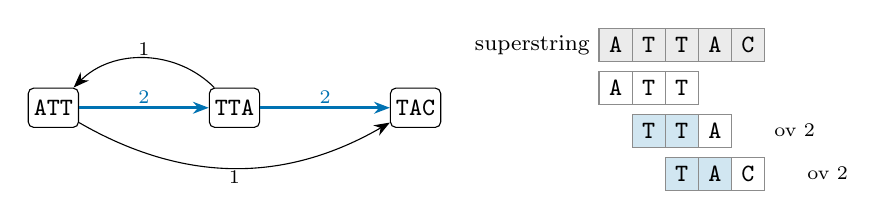
\begin{tikzpicture}[x=0.42cm,y=0.42cm]
  \begin{scope}[x=1cm,y=1cm,shift={(0,-0.8)}]
    \node[vtx,font=\ttfamily\small] (A) at (0,0) {ATT};
    \node[vtx,font=\ttfamily\small] (B) at (2.3,0) {TTA};
    \node[vtx,font=\ttfamily\small] (C) at (4.6,0) {TAC};
    \draw[->,very thick,ocol] (A) -- node[above,ovl]{2} (B);
    \draw[->,very thick,ocol] (B) -- node[above,ovl]{2} (C);
    \draw[->] (A) to[bend right=30] node[below,ovl]{1} (C);
    \draw[->] (B) to[bend right=45] node[above,ovl]{1} (A);
  \end{scope}
  \begin{scope}[shift={(17,0)}]
    \shadecells[black!8]{0}{4}{0}
    \shadecells{1}{2}{-2.6}
    \shadecells{2}{3}{-3.9}
    \cellrow{0}{0}{A,T,T,A,C}
    \cellrow{0}{-1.3}{A,T,T}
    \cellrow{1}{-2.6}{T,T,A}
    \cellrow{2}{-3.9}{T,A,C}
    \node[slabel] at (-0.6,0) {superstring};
    \node[ovl,anchor=west] at (4.7,-2.6) {ov $2$};
    \node[ovl,anchor=west] at (5.7,-3.9) {ov $2$};
  \end{scope}
\end{tikzpicture}
\caption{Left: the overlap graph of $\{\str{ATT},\str{TTA},\str{TAC}\}$
(edges of weight $0$ omitted); its maximum-weight Hamiltonian path is shown
in blue. Right: merging along that path. Shaded cells are shared with the
string above, so the path saves $2+2$ characters.}\label{fig:overlap-graph}
\end{figure}

Two further edge structures are used later. A \emph{matching} is a set of
edges no two of which share a vertex (ignoring direction), and its weight
is its total overlap. For cycle covers we augment the graph with self-loops, weighted by the
proper self-overlaps $\ov(s,s)$. A \emph{cycle cover} is a set of vertex-disjoint
directed cycles, possibly self-loops $(s,s)$, that together contain every
vertex. Let $W$ be the minimum of $\sum_{(s,t)}\operatorname{pref}(s,t)$
over all cycle covers. Closing an optimal ordering $t_1,\dots,t_n$ into a
single cycle shows
\begin{equation}\label{eq:W}
  W\;\le\;\textstyle\sum_{k=1}^{n-1}\operatorname{pref}(t_k,t_{k+1})
     +\operatorname{pref}(t_n,t_1)
  \;\le\;\textstyle\sum_{k=1}^{n-1}\operatorname{pref}(t_k,t_{k+1})+|t_n|
  \;=\;\OPT.
\end{equation}

\subsection{The greedy algorithm}

Greedy (Algorithm~\ref{alg:greedy}) repeatedly merges a pair of distinct
current strings with maximum overlap. The next lemma shows that it never
needs to look beyond the original overlap graph.

\begin{algorithm}[h]
\caption{Maximum-overlap greedy}\label{alg:greedy}
\begin{algorithmic}[1]
\Require substring-free set $S$
\While{$|S|>1$}
  \State choose distinct $s,t\in S$ maximising $\ov(s,t)$, breaking ties by the rule below
  \State $S \gets (S\setminus\{s,t\}) \cup \{s\oplus t\}$
\EndWhile
\State \Return the unique string in $S$
\end{algorithmic}
\end{algorithm}

\begin{lemma}\label{lem:greedy-graph}
Let $\ov(s,t)$ be maximum over distinct pairs in $S$ and
$S'=(S\setminus\{s,t\})\cup\{s\oplus t\}$. Then $S'$ is substring-free, and
for every $u\in S\setminus\{s,t\}$ we have $\ov(u,s\oplus t)=\ov(u,s)$ and
$\ov(s\oplus t,u)=\ov(t,u)$.
\end{lemma}

\begin{proof}
A suffix of $u$ that is a prefix of $s\oplus t$ and longer than $|s|-1$
would contain $s$ as a substring of $u$, so the longest such suffix is a
proper prefix of $s$; this gives $\ov(u,s\oplus t)=\ov(u,s)$, and the
second identity is symmetric. If $u$ were a substring of $s\oplus t$ but
of neither $s$ nor $t$, it would start inside $s$ after its first
character but before the part shared with $t$, and end after $s$ ends. The
part of $s$ from that start onwards would then be a proper suffix of $s$
and a proper prefix of $u$ longer than $\ov(s,t)$, contradicting
maximality. Finally, $s\oplus t$ cannot be a substring of any $u$, as then
$s$ would be.
\end{proof}

By Lemma~\ref{lem:greedy-graph}, a merged string behaves like a path in
the overlap graph: its overlaps are those of its first vertex (incoming)
and last vertex (outgoing). Greedy is therefore equivalent to scanning the
edges in non-increasing order of overlap and accepting an edge $(s,t)$
whenever $s$ has no accepted outgoing edge, $t$ has no accepted incoming
edge, and the edge closes no cycle. The accepted edges form a Hamiltonian
path, and by Lemma~\ref{lem:perm} greedy's output has length $L$ minus
their total overlap. Different orders among equal-weight edges give
different \emph{valid executions}.

\paragraph{Tie-breaking.}
Algorithm~\ref{alg:greedy} leaves ties open, and the output can depend on
them. A \emph{fixed} rule orders all edges in advance (for example by input
index or lexicographically) and takes the first tied edge; a \emph{random}
rule picks uniformly among the tied edges (Section~\ref{sec:experiments}
lists the rules we implement). Unless stated otherwise, theoretical
guarantees in this report hold for \emph{every} valid execution, whereas
lower-bound constructions need only exhibit \emph{one} bad execution.
The two views agree in the worst case: Nikolaev~\cite{Nik21} showed that
every fixed rule has the same worst-case ratio, because an input can be
perturbed so that its overlaps become distinct and a chosen execution is
forced, at almost the same ratio. A particular rule may still avoid the bad
execution on the original input, as Section~\ref{sec:experiments} shows.

\subsection{Measuring solution quality}

Let $\GR$ be the length of greedy's output. Its \emph{length ratio} is
$\GR/\OPT$, and the \emph{worst-case ratio} of greedy is
\[
  \rho=\sup_{S,\;\tau}\;\frac{\GR(S,\tau)}{\OPT(S)},
\]
taken over all instances $S$ and all valid executions $\tau$. The
\emph{compression} of a superstring $w$ is $L-|w|$, the number of
characters saved over concatenation; by Lemma~\ref{lem:perm} the optimal
compression $L-\OPT$ is the weight of a maximum Hamiltonian path. Greedy's
\emph{compression ratio} is $(L-\GR)/(L-\OPT)$ when $L>\OPT$;
when $L=\OPT$, there is no possible compression and we set this ratio to $1$.

The two measures can differ greatly. A compression guarantee
$L-\GR\ge\frac12(L-\OPT)$ only yields $\GR\le\frac12(L+\OPT)$, which can be
far above $2\cdot\OPT$ when $L\gg\OPT$: for $L=100$ and $\OPT=20$ it allows
$\GR=60=3\cdot\OPT$. A constant compression ratio therefore does not by
itself bound the length ratio by any constant.

% =====================================================================
\section{Greedy Achieves Half the Optimal Compression}\label{sec:compression}
% =====================================================================

\begin{theorem}[\cite{TU88,Tur89}]\label{thm:half}
For every substring-free $S$ and valid greedy execution,
$L-\GR \ge \frac12 (L-\OPT)$.
\end{theorem}
 
The original proof of Tarhio and Ukkonen~\cite{TU88} relies on a detailed
case analysis of how an optimal path in the overlap graph can be modified.
Kalugin and Nikolaev~\cite{KN24} proposed a simpler two-part strategy: the
maximum Hamiltonian path weighs at most twice a maximum-weight matching (a
classical observation), and greedy's total overlap is at least that of a
maximum-weight matching. We present our own proof following this
strategy.\footnote{The full text of~\cite{KN24} was not available to us.
The two-part strategy is as described in its abstract; the proofs of
Lemmas~\ref{lem:two-matchings}--\ref{lem:greedy-matching} below are our
own, with Lemma~\ref{lem:monge} taken from~\cite{TU88}.} Write $\ov(M)$ for the total overlap of a set of edges $M$, and $\mu(S)$
for the maximum of $\ov(M)$ over all matchings $M$ of the overlap graph of
$S$. Theorem~\ref{thm:half} follows from two inequalities,
\[
  L-\OPT \;\le\; 2\,\mu(S) \qquad\text{and}\qquad L-\GR \;\ge\; \mu(S).
\]
 
\subsection{From an optimal ordering to two matchings}
 
\begin{lemma}[classical]\label{lem:two-matchings}
$L-\OPT\le 2\,\mu(S)$.
\end{lemma}
 
\begin{proof}
Take an optimal ordering $t_1,\dots,t_n$ and its path edges
$f_k=(t_k,t_{k+1})$, so that $\sum_k\ov(f_k)=L-\OPT$ by
Lemma~\ref{lem:perm}. Colour the edges alternately: $M_1=\{f_1,f_3,\dots\}$
and $M_2=\{f_2,f_4,\dots\}$. Two edges of the same colour, $f_k$ and
$f_{k+2j}$ with $j\ge1$, involve the four distinct vertices $t_k$,
$t_{k+1}$, $t_{k+2j}$, $t_{k+2j+1}$, so each $M_i$ is a matching. As
$\ov(M_1)+\ov(M_2)=L-\OPT$, one of them has weight at least
$\frac12(L-\OPT)$ (Figure~\ref{fig:two-matchings}).
\end{proof}

\begin{figure}[htb]\centering
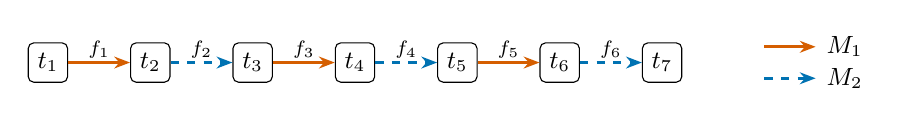
\begin{tikzpicture}[x=1.3cm]
  \foreach \i in {1,...,7} \node[vtx] (t\i) at (\i,0) {$t_{\i}$};
  \foreach \i/\j in {1/2,3/4,5/6}
    \draw[->,very thick,gcol] (t\i) -- node[above,ovl,text=black]{$f_{\i}$} (t\j);
  \foreach \i/\j in {2/3,4/5,6/7}
    \draw[->,very thick,ocol,dashed] (t\i) -- node[above,ovl,text=black]{$f_{\i}$} (t\j);
  \draw[->,very thick,gcol] (8,0.2) -- (8.5,0.2) node[right,font=\small,text=black]{$M_1$};
  \draw[->,very thick,ocol,dashed] (8,-0.2) -- (8.5,-0.2) node[right,font=\small,text=black]{$M_2$};
\end{tikzpicture}
\caption{Lemma~\ref{lem:two-matchings}: the edges of an optimal ordering
alternate between two matchings $M_1$ (solid) and $M_2$ (dashed). Together
they carry all of the overlap $L-\OPT$, so one of them carries at least
half.}\label{fig:two-matchings}
\end{figure}
 
\subsection{Greedy saves at least a maximum-weight matching}
 
The key tool is an exchange property of overlaps: when $(s,t)$ has the
largest overlap, swapping partners never gains more than it loses.
 
\begin{lemma}[Monge inequality {\cite[Lemma~3.1]{TU88}}]\label{lem:monge}
Let $s,t,s',t'\in S$ with $\ov(s,t)\ge\ov(s,t')$ and
$\ov(s,t)\ge\ov(s',t)$. Then $\ov(s,t)+\ov(s',t')\ge\ov(s,t')+\ov(s',t)$.
\end{lemma}
 
\begin{proof}
Let $c=\ov(s,t)$, $a=\ov(s,t')$, $b=\ov(s',t)$, and let $x$ be the
length-$c$ suffix of $s$, which is also the prefix of $t$. If $a+b\le c$
there is nothing to prove. Otherwise, since $a,b\le c$, the length-$b$
suffix of $s'$ is $x[1..b]$ and the length-$a$ prefix of $t'$ is
$x[c-a+1..c]$. Their common part $x[c-a+1..b]$, of length $a+b-c$, is
therefore a suffix of $s'$ and a prefix of $t'$. It is proper, because
$a+b-c\le\min\{a,b\}$, $b<|s'|$ and $a<|t'|$. Hence $\ov(s',t')\ge a+b-c$.
\end{proof}

\begin{figure}[htb]\centering
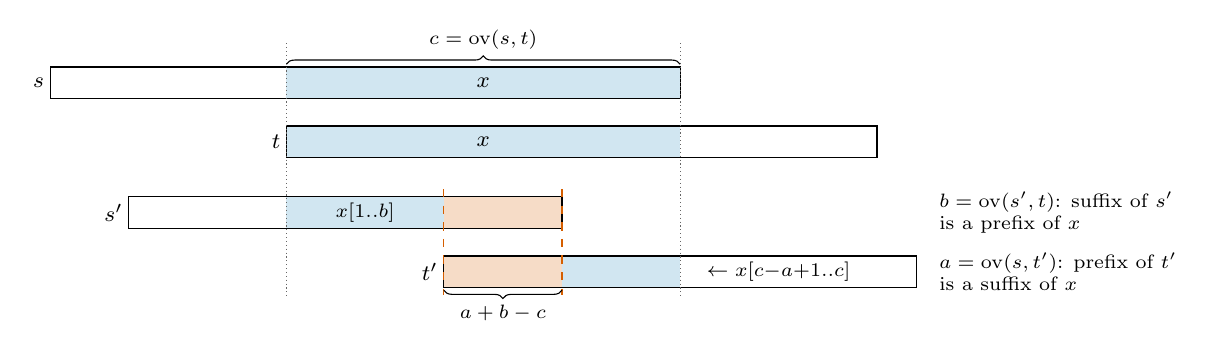
\begin{tikzpicture}[x=0.5cm,y=0.5cm]
  \def\bh{0.4}
  % bars: s, t, s', t'
  \fill[ovfill] (0,-\bh) rectangle (10,\bh);
  \draw (-6,-\bh) rectangle (10,\bh);
  \fill[ovfill] (0,-1.5-\bh) rectangle (10,-1.5+\bh);
  \draw (0,-1.5-\bh) rectangle (15,-1.5+\bh);
  \fill[ovfill] (0,-3.3-\bh) rectangle (7,-3.3+\bh);
  \fill[ovfill] (4,-4.8-\bh) rectangle (10,-4.8+\bh);
  \fill[badfill] (4,-3.3-\bh) rectangle (7,-3.3+\bh);
  \fill[badfill] (4,-4.8-\bh) rectangle (7,-4.8+\bh);
  \draw (-4,-3.3-\bh) rectangle (7,-3.3+\bh);
  \draw (4,-4.8-\bh) rectangle (16,-4.8+\bh);
  % guides
  \draw[densely dotted,black!60] (0,1) -- (0,-5.4) (10,1) -- (10,-5.4);
  \draw[dashed,gcol] (4,-2.7) -- (4,-5.4) (7,-2.7) -- (7,-5.4);
  % labels
  \node[slabel] at (-6,0) {$s$};
  \node[slabel] at (0,-1.5) {$t$};
  \node[slabel] at (-4,-3.3) {$s'$};
  \node[slabel] at (4,-4.8) {$t'$};
  \node[font=\footnotesize] at (5,0) {$x$};
  \node[font=\footnotesize] at (5,-1.5) {$x$};
  \node[font=\scriptsize] at (2,-3.3) {$x[1..b]$};
  \node[font=\scriptsize] at (12.5,-4.8) {$\leftarrow x[c{-}a{+}1..c]$};
  \draw[brc] (0,\bh) -- node[above=5pt,ovl]{$c=\ov(s,t)$} (10,\bh);
  \draw[brc] (7,-4.8-\bh) -- node[below=5pt,ovl]{$a+b-c$} (4,-4.8-\bh);
  \node[ovl,anchor=west,align=left] at (16.5,-3.3)
     {$b=\ov(s',t)$: suffix of $s'$\\ is a prefix of $x$};
  \node[ovl,anchor=west,align=left] at (16.5,-4.8)
     {$a=\ov(s,t')$: prefix of $t'$\\ is a suffix of $x$};
\end{tikzpicture}
\caption{The Monge inequality (Lemma~\ref{lem:monge}). The string $x$ of
length $c$ ends $s$ and begins $t$. If $a+b>c$, the suffix of $s'$ of length
$b$ and the prefix of $t'$ of length $a$ are both pieces of $x$, and they
share the piece $x[c-a+1..b]$ (orange), so $\ov(s',t')\ge a+b-c$.}\label{fig:monge}
\end{figure}
 
\begin{lemma}\label{lem:greedy-matching}
For every substring-free $S$ and every valid greedy execution,
$L-\GR\ge\mu(S)$.
\end{lemma}
 
\begin{proof}
By induction on $n$; for $n=1$ both sides are $0$. Let $(s,t)$ be greedy's
first merge, $c=\ov(s,t)$, $u=s\oplus t$, and
$S'=(S\setminus\{s,t\})\cup\{u\}$. By Lemma~\ref{lem:greedy-graph}, $S'$ is
substring-free and its overlaps are exactly those greedy sees next, so the
remaining merges form a valid execution on $S'$ with the same output.
Since $|u|=|s|+|t|-c$, the total length of $S'$ is $L-c$, and induction
gives $L-\GR = c+\bigl((L-c)-\GR\bigr)\ge c+\mu(S')$.
 
It remains to turn any matching $M$ of $S$ into a matching $M'$ of $S'$
with $\ov(M')\ge\ov(M)-c$. Keep every edge of $M$ that avoids $s$ and $t$.
Recall that $c$ is at least every overlap in $S$, and that by
Lemma~\ref{lem:greedy-graph} an edge into $s$ or out of $t$ keeps its
weight when that endpoint is replaced by $u$:
$\ov(x,u)=\ov(x,s)$ and $\ov(u,y)=\ov(t,y)$.
\begin{itemize}
  \item \emph{At most one edge of $M$ touches $\{s,t\}$} (including
        $(s,t)$ or $(t,s)$ itself). Delete it; it weighs at most $c$.
  \item \emph{$M$ contains $(s,t')$ and $(s',t)$.} Replace both by
        $(s',t')$, where $s'\neq t'$ because $M$ is a matching. By
        Lemma~\ref{lem:monge} the weight drops by at most $c$.
  \item \emph{Otherwise} $M$ has one edge at $s$ and one at $t$, and at
        least one of them enters $s$ or leaves $t$. Keep that edge with $u$
        in place of $s$ or $t$ (same weight) and delete the other edge
        (weight at most $c$).
\end{itemize}
In every case $u$ lies on at most one edge of $M'$, so $M'$ is a matching
of $S'$ and $\ov(M')\ge\ov(M)-c$ (Figure~\ref{fig:matching-cases}). Taking
$M$ of weight $\mu(S)$ gives $\mu(S')\ge\mu(S)-c$, and so $L-\GR\ge\mu(S)$.
\end{proof}

\begin{figure}[htb]\centering
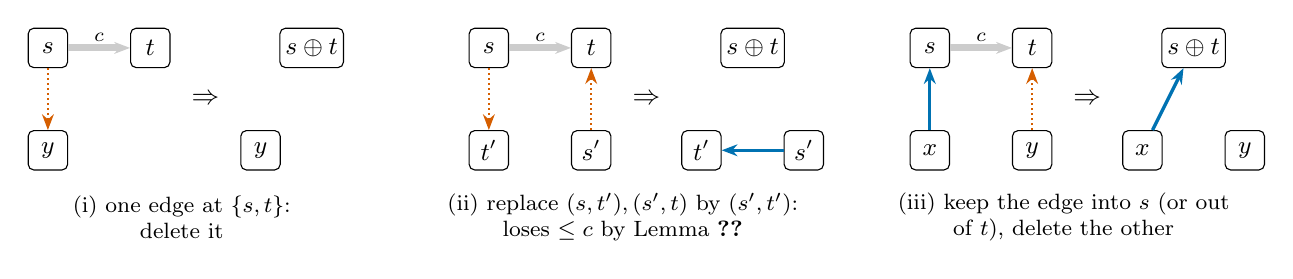
\begin{tikzpicture}[x=1cm,y=1cm]
  \tikzset{merge/.style={line width=2.5pt,black!20},
           kept/.style={->,very thick,ocol},
           gone/.style={->,thick,gcol,densely dotted}}
  % ---- case (i)
  \begin{scope}
    \node[vtx] (s) at (0,0) {$s$}; \node[vtx] (t) at (1.3,0) {$t$};
    \node[vtx] (y) at (0,-1.3) {$y$};
    \draw[merge,->] (s) -- node[above,ovl,text=black]{$c$} (t);
    \draw[gone] (s) -- (y);
    \node at (2,-0.65) {$\Rightarrow$};
    \node[vtx] (u) at (3.35,0) {$s\oplus t$}; \node[vtx] (y2) at (2.7,-1.3) {$y$};
    \node[align=center,font=\footnotesize] at (1.7,-2.15)
      {(i) one edge at $\{s,t\}$:\\ delete it};
  \end{scope}
  % ---- case (ii)
  \begin{scope}[xshift=5.6cm]
    \node[vtx] (s) at (0,0) {$s$}; \node[vtx] (t) at (1.3,0) {$t$};
    \node[vtx] (tp) at (0,-1.3) {$t'$}; \node[vtx] (sp) at (1.3,-1.3) {$s'$};
    \draw[merge,->] (s) -- node[above,ovl,text=black]{$c$} (t);
    \draw[gone] (s) -- (tp); \draw[gone] (sp) -- (t);
    \node at (2,-0.65) {$\Rightarrow$};
    \node[vtx] (u) at (3.35,0) {$s\oplus t$};
    \node[vtx] (tp2) at (2.7,-1.3) {$t'$}; \node[vtx] (sp2) at (4,-1.3) {$s'$};
    \draw[kept] (sp2) -- (tp2);
    \node[align=center,font=\footnotesize] at (1.7,-2.15)
      {(ii) replace $(s,t'),(s',t)$ by $(s',t')$:\\ loses $\le c$ by Lemma~\ref{lem:monge}};
  \end{scope}
  % ---- case (iii)
  \begin{scope}[xshift=11.2cm]
    \node[vtx] (s) at (0,0) {$s$}; \node[vtx] (t) at (1.3,0) {$t$};
    \node[vtx] (x) at (0,-1.3) {$x$}; \node[vtx] (y) at (1.3,-1.3) {$y$};
    \draw[merge,->] (s) -- node[above,ovl,text=black]{$c$} (t);
    \draw[kept] (x) -- (s); \draw[gone] (y) -- (t);
    \node at (2,-0.65) {$\Rightarrow$};
    \node[vtx] (u) at (3.35,0) {$s\oplus t$};
    \node[vtx] (x2) at (2.7,-1.3) {$x$}; \node[vtx] (y2) at (4,-1.3) {$y$};
    \draw[kept] (x2) -- (u);
    \node[align=center,font=\footnotesize] at (1.7,-2.15)
      {(iii) keep the edge into $s$ (or out\\ of $t$), delete the other};
  \end{scope}
\end{tikzpicture}
\caption{Turning a matching $M$ of $S$ into a matching $M'$ of $S'$ after
greedy merges $(s,t)$ with the maximum overlap $c$ (proof of
Lemma~\ref{lem:greedy-matching}). Dotted edges are deleted, blue edges are
kept or created. Each case loses at most $c$, because no edge weighs more
than $c$ and edges into $s$ or out of $t$ keep their weight
(Lemma~\ref{lem:greedy-graph}).}\label{fig:matching-cases}
\end{figure}
 
\subsection{Consequences and limitations}

\begin{proof}[Proof of Theorem~\ref{thm:half}]
By Lemmas~\ref{lem:greedy-matching} and~\ref{lem:two-matchings}, 
\[L-\GR\ge\mu(S)\ge\frac12(L-\OPT).\qedhere\]
\end{proof}


The factor $\frac12$ is tight, as the following example shows. For an integer $h\ge1$ and
distinct symbols $\str{a},\str{b},\str{c}$, let
\[
S_h=\{\str{a}\str{b}^h,\;\str{b}^{h+1},\;
       \str{b}^h\str{c}\}.
\]
The three overlaps $\ov(\str{a}\str{b}^h,\str{b}^{h+1}),
\ov(\str{b}^{h+1},\str{b}^h\str{c}),
\ov(\str{a}\str{b}^h,\str{b}^h\str{c})$
all have the maximum value $h$. Greedy may therefore first merge
$\str{a}\str{b}^h$ with $\str{b}^h\str{c}$, producing
$\str{a}\str{b}^h\str{c}$. This merged string has no nonempty
overlap with $\str{b}^{h+1}$ in either direction, so the final
output has length $\GR=2h+3$. Meanwhile, $\str{a}\str{b}^{h+1}\str{c}$ is an optimal
superstring of length $h+3$: every feasible solution must contain
at least $h+1$ copies of $\str{b}$, together with $\str{a}$ and
$\str{c}$. Since $L=3h+3$,
\[
\frac{L-\GR}{L-\OPT}=\frac{h}{2h}=\frac12.
\]
Thus no larger compression factor can hold for every valid greedy
execution. The same family also satisfies
\[
\frac{\GR}{\OPT}=\frac{2h+3}{h+3}\longrightarrow 2,
\]
giving the classical lower bound for the length ratio discussed
in Section~\ref{sec:worstcase}. Figure~\ref{fig:Sh} shows both
superstrings for $h=3$.

\begin{figure}[htb]\centering
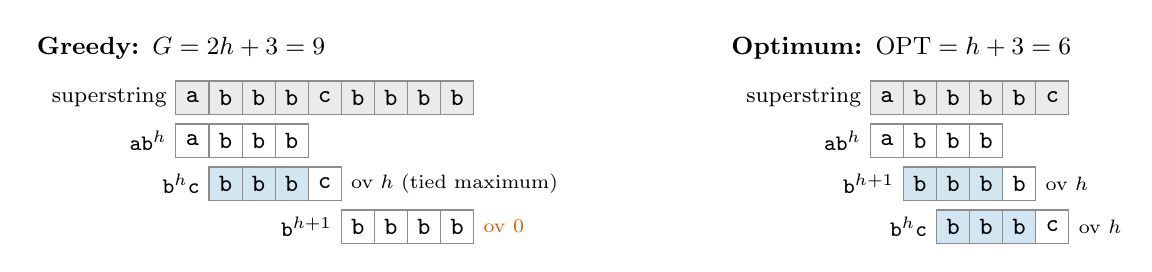
\begin{tikzpicture}[x=0.42cm,y=0.42cm]
  % greedy
  \node[panel] at (-5,1.5) {Greedy: $\GR=2h+3=9$};
  \shadecells[black!8]{0}{8}{0}
  \shadecells{1}{3}{-2.6}
  \cellrow{0}{0}{a,b,b,b,c,b,b,b,b}
  \cellrow{0}{-1.3}{a,b,b,b}
  \cellrow{1}{-2.6}{b,b,b,c}
  \cellrow{5}{-3.9}{b,b,b,b}
  \node[slabel] at (-0.6,0) {superstring};
  \node[slabel] at (-0.6,-1.3) {$\str{a}\str{b}^h$};
  \node[slabel] at (0.4,-2.6) {$\str{b}^h\str{c}$};
  \node[slabel] at (4.4,-3.9) {$\str{b}^{h+1}$};
  \node[ovl,anchor=west] at (4.7,-2.6) {ov $h$ (tied maximum)};
  \node[ovl,anchor=west,text=gcol] at (8.7,-3.9) {ov $0$};
  % optimum
  \begin{scope}[shift={(21,0)}]
  \node[panel] at (-5,1.5) {Optimum: $\OPT=h+3=6$};
  \shadecells[black!8]{0}{5}{0}
  \shadecells{1}{3}{-2.6}
  \shadecells{2}{4}{-3.9}
  \cellrow{0}{0}{a,b,b,b,b,c}
  \cellrow{0}{-1.3}{a,b,b,b}
  \cellrow{1}{-2.6}{b,b,b,b}
  \cellrow{2}{-3.9}{b,b,b,c}
  \node[slabel] at (-0.6,0) {superstring};
  \node[slabel] at (-0.6,-1.3) {$\str{a}\str{b}^h$};
  \node[slabel] at (0.4,-2.6) {$\str{b}^{h+1}$};
  \node[slabel] at (1.4,-3.9) {$\str{b}^h\str{c}$};
  \node[ovl,anchor=west] at (4.7,-2.6) {ov $h$};
  \node[ovl,anchor=west] at (5.7,-3.9) {ov $h$};
  \end{scope}
\end{tikzpicture}
\caption{The tight family $S_h$ for $h=3$. Shaded cells are shared with the
string above. All three non-zero overlaps equal $h$, and greedy may merge
$\str{a}\str{b}^h$ with $\str{b}^h\str{c}$ first; the merged string has no
overlap with $\str{b}^{h+1}$, so greedy saves $h$ characters where the
optimum saves $2h$.}\label{fig:Sh}
\end{figure}

Uniform random tie-breaking selects the bad merge with probability $1/3$;
reordering can make index-based rules select it too.
Theorem~\ref{thm:half} only implies $\GR\le(L+\OPT)/2$. Since $L/\OPT$
is unbounded, this gives no constant length guarantee and motivates the
cycle-cover analysis in Section~\ref{sec:worstcase}.

\begin{comment}
\begin{proof}[Proof of Theorem~\ref{thm:half}]
By Lemmas~\ref{lem:greedy-matching} and~\ref{lem:two-matchings},
$L-\GR\ge\mu(S)\ge\frac12(L-\OPT)$.
\end{proof}
 
The factor $\frac12$ cannot be improved, as the following example shows. For $h\ge1$ let
$S_h=\{\str{a}\str{b}^h,\;\str{b}^{h+1},\;\str{b}^h\str{c}\}$. The overlaps
$\ov(\str{ab}^h,\str{b}^{h+1})$, $\ov(\str{b}^{h+1},\str{b}^h\str{c})$ and
$\ov(\str{ab}^h,\str{b}^h\str{c})$ all equal the maximum $h$, so greedy may
first merge $\str{ab}^h$ with $\str{b}^h\str{c}$. Only this one of the
three tied choices is bad: the fixed rules of Section~\ref{sec:experiments}
all avoid it, and random tie-breaking makes it with probability $1/3$. 
The result $\str{ab}^h\str{c}$ has no overlap with $\str{b}^{h+1}$ in either
direction, so $L-\GR=h$, whereas the optimum $\str{ab}^{h+1}\str{c}$ saves
$2h$. The same instances give $\GR/\OPT=(2h+3)/(h+3)\to 2$, the classical
lower bound for the length ratio discussed in Section~\ref{sec:worstcase}.
 
Compared with the classical argument, which forces the edge $(s,t)$ into
an optimal path and loses up to $2c$ per merge through path rerouting (see
Fici et al.~\cite{FKRRW16} for this argument in a variant of SCS), the
matching argument loses only $c$ per merge and needs no rerouting: the
factor $\frac12$ is paid once, in Lemma~\ref{lem:two-matchings}.
 
For length, Theorem~\ref{thm:half} only yields $\GR\le\frac12(L+\OPT)$,
which, as noted in Section~\ref{sec:prelim}, is not bounded by any constant
multiple of $\OPT$. The matching argument compares greedy with $L$ rather
than with $\OPT$ and discards the order in which strings are chained.
Bounding the length ratio requires a finer comparison with the structure
of an optimal solution; this is the role of cycle covers in
Section~\ref{sec:worstcase}.
\end{comment}
% =====================================================================
\section{The Worst-Case Length Ratio of Greedy}\label{sec:worstcase}
% =====================================================================

\subsection{The greedy conjecture: history and current bounds}
\label{sec:greedy-history}

The greedy algorithm repeatedly merges an ordered pair of strings with
maximum suffix--prefix overlap. Its simplicity contrasts with the difficulty
of bounding the length of its output. In 1988, Tarhio and
Ukkonen~\cite{TU88} formulated the following conjecture.

\begin{conjecture}[Historical greedy superstring conjecture]
For every substring-free input set $S$ and every valid greedy execution,
$\GR(S)\le 2\OPT(S)$.
\end{conjecture}

Examples approaching ratio $2$ were already known; Section~\ref{sec:lower-two}
gives one with only three strings. Thus the conjectured factor, if true,
would have been tight. Proving an upper bound was much harder. Blum et
al.~\cite{BJLTY94} obtained the first constant bound, namely $4$, in work
first presented at STOC 1991 and expanded in 1994. Subsequent improvements
for the original greedy algorithm were as follows:
\begin{center}
\begin{tabular}{lll}
\toprule
Year & Upper bound on $\GR/\OPT$ & Reference \\
\midrule
1991/1994 & $4$ & Blum et al.~\cite{BJLTY94} \\
2005 & $7/2$ & Kaplan and Shafrir~\cite{KS05} \\
2022 & $(13+\sqrt{57})/6$ & Englert et al.~\cite{EMV22} \\
2023 & $(2+\sqrt{67})/3$ & Englert et al.~\cite{EMV23} \\
2026 & $3$ & Chukhin et al.~\cite{CKMS26} \\
\bottomrule
\end{tabular}
\end{center}

The conjecture was finally disproved in 2026. Shibata's original
preprint~\cite{Shi26} established a lower bound of $9/4$ on the worst-case
ratio. The subsequent joint paper by Chukhin et al.~\cite{GSC26} improved
this lower bound to $12/5$. Consequently, if $\rho_{\mathrm{greedy}}$
denotes the supremum of $\GR(S)/\OPT(S)$ over inputs and valid executions,
the current bounds are
\[
  \frac{12}{5}\le\rho_{\mathrm{greedy}}\le3.
\]
Section~\ref{sec:upper-three} explains the upper bound. The elementary
family below illustrates the earlier lower bound of $2$; the constructions
exceeding $2$ require additional ideas.

\subsection{An elementary family approaching ratio two}
\label{sec:lower-two}

Let $a,b,c$ be distinct characters. For each integer $k\ge1$, consider
the classical family~\cite{BJLTY94}
\[
  S_k=\{x_k,y_k,z_k\},\qquad
  x_k=c(ab)^k,\quad y_k=(ba)^k,\quad z_k=(ab)^kc.
\]
The total input length is $L=6k+2$. The directed overlaps between distinct
strings are
\[
\begin{array}{c|ccc}
  \ov(\cdot,\cdot) & x_k & y_k & z_k\\ \hline
  x_k & - & 2k-1 & 2k\\
  y_k & 0 & - & 2k-1\\
  z_k & 1 & 0 & -
\end{array}
\]
The unique maximum overlap is from $x_k$ to $z_k$, so greedy must first
merge them into $c(ab)^kc$. This string starts and ends with $c$, whereas
$y_k$ contains no $c$, so the remaining two strings have no overlap in
either direction. Every valid execution therefore has length
\[
  \GR(S_k)=(2k+2)+2k=4k+2.
\]

In contrast, the order $x_k,y_k,z_k$ saves $2(2k-1)$ characters and gives
the superstring $c(ab)^{k+1}c$, of length $2k+4$. The overlap table also
proves optimality: a Hamiltonian path using $x_k\to z_k$ has total overlap
$2k$, while one avoiding that edge has total overlap at most $4k-2$.
Since $2k\le4k-2$, the maximum is $4k-2$, attained by
$x_k\to y_k\to z_k$. Hence
\[
  \OPT(S_k)=L-(4k-2)=2k+4,
  \qquad
  \frac{\GR(S_k)}{\OPT(S_k)}
  =\frac{4k+2}{2k+4}
  =2-\frac{6}{2k+4}\longrightarrow2.
\]
Thus no approximation guarantee strictly smaller than $2$ is possible
for greedy. This family approaches $2$ from below and does not itself
disprove the historical conjecture. It shows how taking the largest
single overlap can prevent two almost-as-large overlaps from being used
(Figure~\ref{fig:Sk}).

\begin{figure}[htb]\centering
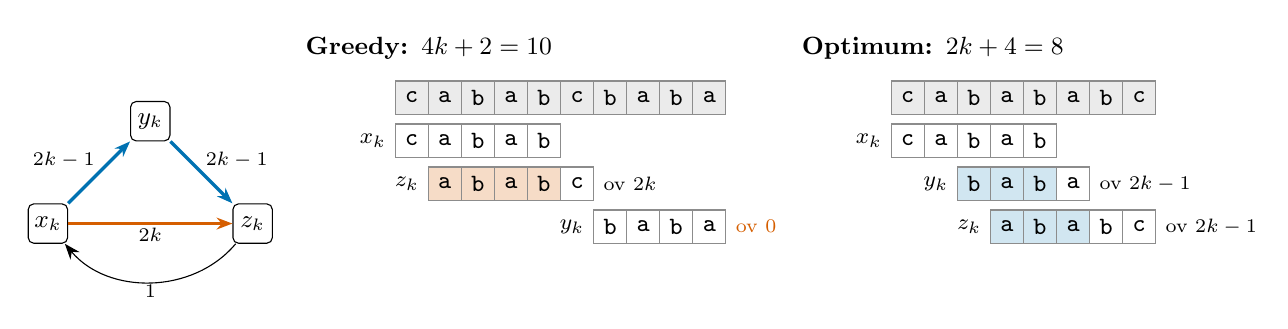
\begin{tikzpicture}[x=0.42cm,y=0.42cm]
  \begin{scope}[x=1cm,y=1cm,shift={(0,-1.6)}]
    \node[vtx] (x) at (0,0) {$x_k$};
    \node[vtx] (y) at (1.3,1.3) {$y_k$};
    \node[vtx] (z) at (2.6,0) {$z_k$};
    \draw[->,very thick,gcol] (x) -- node[below,ovl,text=black]{$2k$} (z);
    \draw[->,very thick,ocol] (x) -- node[above left,ovl,text=black]{$2k-1$} (y);
    \draw[->,very thick,ocol] (y) -- node[above right,ovl,text=black]{$2k-1$} (z);
    \draw[->] (z) to[bend left=50] node[below,ovl]{$1$} (x);
  \end{scope}
  % greedy
  \begin{scope}[shift={(11,0)}]
    \node[panel] at (-3.5,1.5) {Greedy: $4k+2=10$};
    \shadecells[black!8]{0}{9}{0}
    \shadecells[badfill]{1}{4}{-2.6}
    \cellrow{0}{0}{c,a,b,a,b,c,b,a,b,a}
    \cellrow{0}{-1.3}{c,a,b,a,b}
    \cellrow{1}{-2.6}{a,b,a,b,c}
    \cellrow{6}{-3.9}{b,a,b,a}
    \node[slabel] at (-0.6,-1.3) {$x_k$};
    \node[slabel] at (0.4,-2.6) {$z_k$};
    \node[slabel] at (5.4,-3.9) {$y_k$};
    \node[ovl,anchor=west] at (5.7,-2.6) {ov $2k$};
    \node[ovl,anchor=west,text=gcol] at (9.7,-3.9) {ov $0$};
  \end{scope}
  % optimum
  \begin{scope}[shift={(26,0)}]
    \node[panel] at (-3.5,1.5) {Optimum: $2k+4=8$};
    \shadecells[black!8]{0}{7}{0}
    \shadecells{2}{4}{-2.6}
    \shadecells{3}{5}{-3.9}
    \cellrow{0}{0}{c,a,b,a,b,a,b,c}
    \cellrow{0}{-1.3}{c,a,b,a,b}
    \cellrow{2}{-2.6}{b,a,b,a}
    \cellrow{3}{-3.9}{a,b,a,b,c}
    \node[slabel] at (-0.6,-1.3) {$x_k$};
    \node[slabel] at (1.4,-2.6) {$y_k$};
    \node[slabel] at (2.4,-3.9) {$z_k$};
    \node[ovl,anchor=west] at (5.7,-2.6) {ov $2k-1$};
    \node[ovl,anchor=west] at (7.7,-3.9) {ov $2k-1$};
  \end{scope}
\end{tikzpicture}
\caption{The family $S_k$ of Section~\ref{sec:lower-two}. Left: its overlap
graph (edges of weight $0$ omitted). The unique maximum edge $x_k\to z_k$
(vermillion) is taken first and blocks the path $x_k\to y_k\to z_k$
(blue). Right: the two superstrings for $k=2$; shaded cells are shared with
the string above.}\label{fig:Sk}
\end{figure}

\subsection{A 3-approximation guarantee for greedy}
\label{sec:upper-three}

Chukhin et al.~\cite{CKMS26} proved that every valid greedy execution
satisfies $\GR\le 3\OPT$. The main ingredient is a bound on the overlap
lost when opening the cycles of an optimal cycle cover. We prove this
bound below, then invoke the classical analysis of Blum et
al.~\cite{BJLTY94} to obtain the guarantee for the original greedy algorithm.

\paragraph{Cycle covers and periodic words.}
Let $\mathcal C$ be a minimum-prefix-cost cycle cover. For a cycle
$C=(t_1,\ldots,t_r,t_1)$, with $t_{r+1}=t_1$, put
\[
  w(C)=\sum_{i=1}^{r}\operatorname{pref}(t_i,t_{i+1}),
  \qquad
  o(C)=\min_{1\le i\le r}\ov(t_i,t_{i+1}),
  \qquad
  O=\sum_{C\in\mathcal C}o(C).
\]
Thus $W=\sum_C w(C)\le\OPT$. Opening $C$ at an edge of minimum overlap
produces a representative string $\sigma(C)$ of length $w(C)+o(C)$.
Concatenating these representatives, as MGREEDY does, gives length $W+O$.

To distinguish prefix strings from their lengths, let $p(s,t)$ be the
prefix of $s$ of length $\operatorname{pref}(s,t)$. Fix a total order on
$\Sigma$. Define the cycle word
$\tau(C)=p(t_1,t_2)\cdots p(t_r,t_1)$, so $|\tau(C)|=w(C)$.
A word is \emph{primitive} if it is not a power of a shorter word; its
lexicographically smallest rotation is then a \emph{Lyndon word}.
A Lyndon word has no period smaller than its length.
The cycle words of $\mathcal C$ are primitive and pairwise distinct up
to rotation~\cite[Lemma 2.5]{Muc13}. Their Lyndon representatives $z_C$
are therefore distinct, with $|z_C|=w(C)$.

Write $\operatorname{Sub}_m(u)$ for the set of distinct length-$m$
substrings of $u$, and $\operatorname{CSub}_m(z)$ for those of the
infinite repetition $z^\infty$, with $\operatorname{Sub}_0(u)=\{\varepsilon\}$.
A classical periodicity property~\cite{BJLTY94} gives, for any common
superstring $T$,
\begin{equation}\label{eq:upper-forced-windows}
  \operatorname{CSub}_{o(C)+1}(z_C)
  \subseteq \operatorname{Sub}_{o(C)+1}(T).
\end{equation}
Indeed, unfold the cycle periodically. If consecutive input occurrences
start at positions $a<b$, the first ends at or after $b+o(C)-1$
(using inclusive end positions).
Every length-$(o(C)+1)$ window starting at $a,\ldots,b-1$ lies in that
input occurrence. These intervals cover all starting positions in the
periodic text. The same inclusion holds for every shorter window length
(Figure~\ref{fig:cycles}, left).

\begin{figure}[htb]\centering
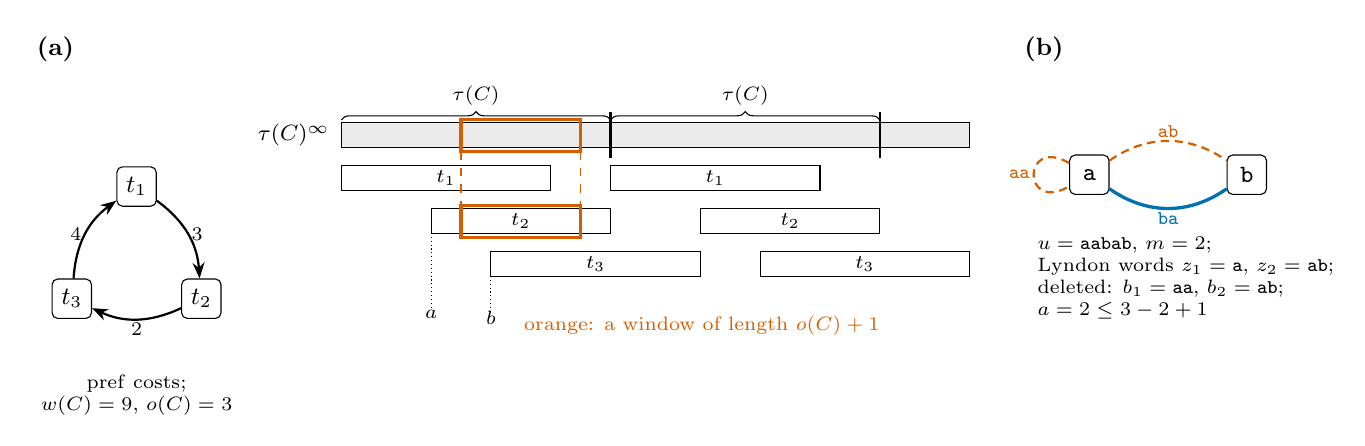
\begin{tikzpicture}[x=0.38cm,y=0.42cm]
  \node[panel] at (-10.5,2.6) {(a)};
  % the cycle
  \begin{scope}[x=1cm,y=1cm,shift={(-2.6,-1.6)}]
    \node[vtx] (a) at (90:0.95) {$t_1$};
    \node[vtx] (b) at (330:0.95) {$t_2$};
    \node[vtx] (c) at (210:0.95) {$t_3$};
    \draw[->,thick] (a) to[bend left=25] node[right,ovl]{$3$} (b);
    \draw[->,thick] (b) to[bend left=25] node[below,ovl]{$2$} (c);
    \draw[->,thick] (c) to[bend left=25] node[left,ovl]{$4$} (a);
    \node[ovl,align=center] at (0,-1.7) {$\operatorname{pref}$ costs;\\ $w(C)=9$, $o(C)=3$};
  \end{scope}
  % unfolded text
  \def\bh{0.38}
  \fill[black!8] (0,-\bh) rectangle (21,\bh);
  \draw (0,-\bh) rectangle (21,\bh);
  \foreach \p in {9,18} \draw[thick] (\p,-0.7) -- (\p,0.7);
  \draw[brc] (0,\bh) -- node[above=5pt,ovl]{$\tau(C)$} (9,\bh);
  \draw[brc] (9,\bh) -- node[above=5pt,ovl]{$\tau(C)$} (18,\bh);
  \node[slabel] at (-0.2,0) {$\tau(C)^\infty$};
  \foreach \st/\en/\lab/\row in {0/7/1/1,3/9/2/2,5/12/3/3,9/16/1/1,12/18/2/2,14/21/3/3}{
    \draw[fill=white] (\st,-1.3*\row-\bh) rectangle (\en,-1.3*\row+\bh);
    \node[ovl] at ({(\st+\en)/2},-1.3*\row) {$t_{\lab}$};}
  % a forced window inside the occurrence of t_2
  \draw[gcol,very thick] (4,-\bh-0.1) rectangle (8,\bh+0.1);
  \draw[gcol,very thick] (4,-2.6-\bh-0.1) rectangle (8,-2.6+\bh+0.1);
  \draw[gcol,dashed] (4,-\bh-0.1) -- (4,-2.6+\bh+0.1) (8,-\bh-0.1) -- (8,-2.6+\bh+0.1);
  \draw[densely dotted] (3,-2.6) -- (3,-5.2) node[below,ovl]{$a$};
  \draw[densely dotted] (5,-3.9) -- (5,-5.2) node[below,ovl]{$b$};
  \node[ovl,anchor=west,text=gcol] at (6,-5.75) {orange: a window of length $o(C)+1$};
  % ---- (b) counting graph
  \begin{scope}[shift={(25,0)}]
    \node[panel] at (-2.5,2.6) {(b)};
    \begin{scope}[x=1cm,y=1cm,shift={(0,-0.5)}]
      \node[vtx] (va) at (0,0) {$\str{a}$};
      \node[vtx] (vb) at (2,0) {$\str{b}$};
      \draw[gcol,thick,densely dashed] (va) to[out=150,in=210,looseness=6]
        node[left,ovl]{$\str{aa}$} (va);
      \draw[gcol,thick,densely dashed] (va) to[bend left=35]
        node[above,ovl]{$\str{ab}$} (vb);
      \draw[ocol,very thick] (va) to[bend right=35] node[below,ovl]{$\str{ba}$} (vb);
      \node[ovl,align=left,anchor=north west] at (-0.7,-0.75)
        {$u=\str{aabab}$, $m=2$;\\
         Lyndon words $z_1=\str{a}$, $z_2=\str{ab}$;\\
         deleted: $b_1=\str{aa}$, $b_2=\str{ab}$;\\
         $a=2\le 3-2+1$};
    \end{scope}
  \end{scope}
\end{tikzpicture}
\caption{(a) Unfolding a cycle $C=(t_1,t_2,t_3)$ along its periodic word
$\tau(C)^\infty$. Consecutive occurrences overlap by at least $o(C)$, so
every window of length $o(C)+1$ that starts in $[a,b)$, where $a$ and $b$
are consecutive start positions, lies inside the occurrence starting at
$a$; the window shown starts at $b-1$. (b) The graph in the proof of
Lemma~\ref{lem:upper-periodic-count}: vertices are $\operatorname{Sub}_{m-1}(u)$
and edges are $\operatorname{Sub}_m(u)$. Deleting the smallest label $b_j$ of
each Lyndon word's closed walk (dashed) leaves the graph connected, so at
most $|E|-|V|+1$ edges can be deleted.}\label{fig:cycles}
\end{figure}

\paragraph{Counting periodic patterns.}
The following lemma is the key counting step of~\cite{CKMS26}.

\begin{lemma}\label{lem:upper-periodic-count}
Let $1\le m\le |u|$, and let $z_1,\ldots,z_a$ be distinct Lyndon words
such that $|z_j|\le m$ and
$\operatorname{CSub}_m(z_j)\subseteq\operatorname{Sub}_m(u)$.
Then
\[
  a\le |\operatorname{Sub}_m(u)|
       -|\operatorname{Sub}_{m-1}(u)|+1.
\]
\end{lemma}

\begin{proof}
Construct an undirected multigraph whose vertices are
$\operatorname{Sub}_{m-1}(u)$. Each word in $\operatorname{Sub}_m(u)$
is an edge between its length-$(m-1)$ prefix and suffix; loops are allowed.
Sliding a window through $u$ visits every vertex, so the graph is connected.

For each $j$, choose the length-$m$ prefix $b_j$ of $z_j^\infty$.
Since $m\ge |z_j|$ and $z_j$ is Lyndon, $b_j$ is the unique smallest
edge label in its periodic closed walk. The labels $b_j$ are distinct:
if $b_i=b_j$ and $|z_i|=|z_j|$, their initial letters give $z_i=z_j$.
If $|z_i|<|z_j|$, then $z_j$ is a prefix of $z_i^\infty$ and has period
$|z_i|$, contradicting the Lyndon property.

Delete $b_1,\ldots,b_a$ in increasing lexicographic order. When $b_j$
is deleted, all other edges of its periodic closed walk are larger,
so none has been deleted. They still connect its endpoints; deleting
a loop is harmless. Thus the graph remains connected after all $a$
deletions. The inequality $|E|-a\ge |V|-1$ proves the claim; see
Figure~\ref{fig:cycles}(b) for a small example.
\end{proof}

\paragraph{The cycle-cover inequality.}

\begin{theorem}[\cite{CKMS26}]\label{thm:upper-cycle-inequality}
For the optimal cycle cover above, $O-W\le\OPT$.
\end{theorem}

\begin{proof}
Fix a shortest common superstring $T^\star$ and put
$N=|T^\star|=\OPT$ and $P_m=|\operatorname{Sub}_m(T^\star)|$.
For $1\le m\le N$, define
\[
  a_m=\bigl|\{C\in\mathcal C:w(C)\le m\le o(C)+1\}\bigr|.
\]
The words $z_C$ counted here are distinct Lyndon words of length at most
$m$, and~\eqref{eq:upper-forced-windows} supplies all their length-$m$
windows. Lemma~\ref{lem:upper-periodic-count} therefore gives
$a_m\le P_m-P_{m-1}+1$. Since $P_0=P_N=1$,
\[
  \sum_{m=1}^{N}a_m
  \le \sum_{m=1}^{N}(P_m-P_{m-1}+1)=N.
\]
Each cycle is counted once for each integer in $[w(C),o(C)+1]$.
The upper endpoint is at most $N$ by~\eqref{eq:upper-forced-windows}.
Double counting yields
\[
  O-W
  \le \sum_{C\in\mathcal C}\max\{0,o(C)-w(C)+2\}
  =\sum_{m=1}^{N}a_m
  \le N=\OPT.
\]
\end{proof}

\paragraph{Transferring the bound to greedy.}
The preceding theorem immediately gives the MGREEDY bound
$W+O\le\OPT+2W\le3\OPT$.
For the original greedy algorithm, we use the classical transfer analysis
of Blum et al.~\cite[Section 5]{BJLTY94}: every valid execution on $S$
determines a nonempty subset $U\subseteq S$ and an optimal cycle cover
of $U$ whose quantities $W_U,O_U$ satisfy
\begin{equation}\label{eq:upper-classical-transfer}
  \GR(S)\le 2\OPT(S)+O_U-W_U.
\end{equation}
This is an invoked classical result; Appendix~\ref{app:upper} outlines
its construction using the innermost cycles that greedy refuses to close.

\begin{corollary}[\cite{CKMS26}]
For every substring-free input $S$ and every valid greedy execution,
$\GR(S)\le3\OPT(S)$.
\end{corollary}
\begin{proof}
Apply Theorem~\ref{thm:upper-cycle-inequality} to $U$ and use
$\OPT(U)\le\OPT(S)$ in~\eqref{eq:upper-classical-transfer}:
$\GR(S)\le2\OPT(S)+\OPT(U)\le3\OPT(S)$.
\end{proof}


% =====================================================================
\subsection{A lower bound of \texorpdfstring{$12/5$}{12/5}}\label{sec:lower-twelve-fifths}

We simplify the exposition of Chukhin et al.'s five-string
construction~\cite[Section 4]{GSC26}. Their parameters $r$ and $P$
control group count and gap scale; treating them independently adds
bookkeeping to the overlap comparisons and length formulas. For our
asymptotic lower bound, one sequence suffices: $P=r^2$ makes the leading
$Pr$ terms dominate the $O(r^2+P)$ corrections. The original paper
already uses this scaling to obtain $12/5$. We fix a quadratic scale
and adjust the gap and padding constants below.
Appendix~\ref{app:shibata} verifies this single-parameter adaptation.
For nonnegative integers $L,R$ and positive gaps
$g_1,\ldots,g_k$, use the notation
\[
 [L\mid g_1,\ldots,g_k\mid R]
 =0^L1\,0^{g_1-1}1\cdots0^{g_k-1}1\,0^R.
\]
Its length is $L+R+1+\sum_jg_j$. Fix $n\ge2$, put
$N=n^2$, $M=N+4n$, and $p_i=N+i$ for $2\le i\le n$.
The input $S_n$ consists of the following $5(n-1)$ binary strings:
\begin{center}
\begin{tabular}{cclc}
\toprule
String & Left pad & Gap sequence & Right pad\\
\midrule
$X_i$ & $N+n$ & $p_i,M,p_i,M$ & $N$\\
$Y_i$ & $N$ & $M,p_i,M,p_i$ & $N+2n$\\
$U_i$ & $N$ & $M,M,p_i,M$ & $N$\\
$V_i$ & $N$ & $M,p_i,M,M$ & $N+1$\\
$Z_i$ & $p_i-1$ & $M,M,p_i$ & $0$\\
\bottomrule
\end{tabular}
\end{center}
Figure~\ref{fig:twelve-fifths} shows the notation, how each group of five
strings fits into one short superstring, and the bad greedy merge order.

\begin{figure}[htbp]\centering
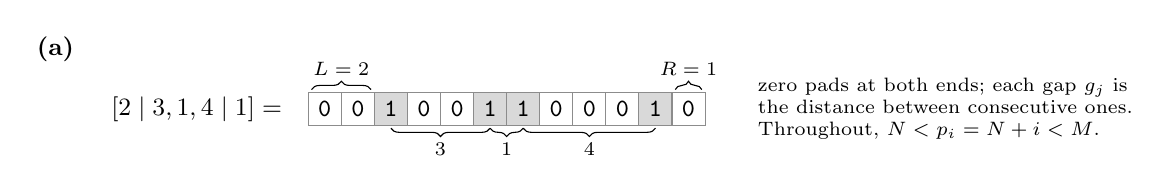
\begin{tikzpicture}[x=0.42cm,y=0.42cm]
  % ---- (a) notation
  \node[panel] at (-9,1.8) {(a)};
  \node[anchor=east,font=\small] at (-1,0) {$[2\mid 3,1,4\mid 1]=$};
  \shadecells[black!15]{2}{2}{0}\shadecells[black!15]{5}{6}{0}\shadecells[black!15]{10}{10}{0}
  \cellrow{0}{0}{0,0,1,0,0,1,1,0,0,0,1,0}
  \draw[brc] (-0.4,0.5) -- node[above=5pt,ovl]{$L=2$} (1.4,0.5);
  \draw[brc] (10.6,0.5) -- node[above=5pt,ovl]{$R=1$} (11.4,0.5);
  \draw[brc] (5,-0.5) -- node[below=5pt,ovl]{$3$} (2,-0.5);
  \draw[brc] (6,-0.5) -- node[below=5pt,ovl]{$1$} (5,-0.5);
  \draw[brc] (10,-0.5) -- node[below=5pt,ovl]{$4$} (6,-0.5);
  \node[ovl,anchor=west,align=left] at (13,0)
    {zero pads at both ends; each gap $g_j$ is\\
     the distance between consecutive ones.\\
     Throughout, $N<p_i=N+i<M$.};
\end{tikzpicture}

\medskip
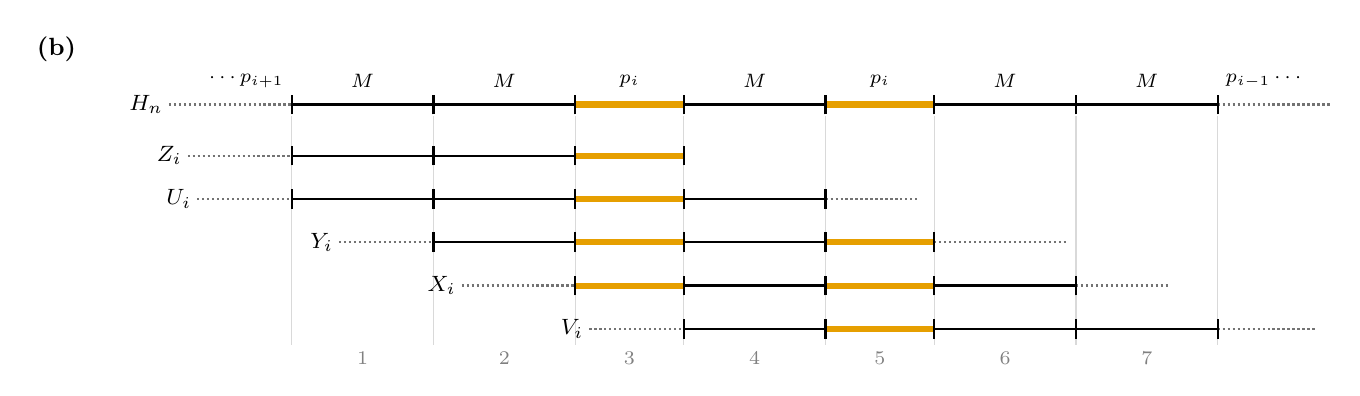
\begin{tikzpicture}[x=0.6cm,y=0.5cm]
  % ---- (b) one group inside H_n (schematic lengths: N=2, p_i=2.3, M=3)
  \node[panel] at (-5.6,1.4) {(b)};
  \foreach \x in {0,3,6,8.3,11.3,13.6,16.6,19.6}
    \draw[black!15] (\x,-0.3) -- (\x,-6.1);
  \gaprow{0}{$H_n$}{-2.6}{0}{19.6}{22}{0,3,6,8.3,11.3,13.6,16.6,19.6}{6/8.3,11.3/13.6}
  \node[ovl,anchor=east] at (-0.1,0.6) {$\cdots p_{i+1}$};
  \node[ovl,anchor=west] at (19.7,0.6) {$p_{i-1}\cdots$};
  \foreach \a/\b/\l in {0/3/M,3/6/M,6/8.3/p_i,8.3/11.3/M,11.3/13.6/p_i,13.6/16.6/M,16.6/19.6/M}
    \node[ovl] at ({(\a+\b)/2},0.6) {$\l$};
  \foreach \a/\b/\l in {0/3/1,3/6/2,6/8.3/3,8.3/11.3/4,11.3/13.6/5,13.6/16.6/6,16.6/19.6/7}
    \node[ovl,text=black!50] at ({(\a+\b)/2},-6.45) {\l};
  \gaprow{-1.3}{$Z_i$}{-2.2}{0}{8.3}{8.3}{0,3,6,8.3}{6/8.3}
  \gaprow{-2.4}{$U_i$}{-2}{0}{11.3}{13.3}{0,3,6,8.3,11.3}{6/8.3}
  \gaprow{-3.5}{$Y_i$}{1}{3}{13.6}{16.4}{3,6,8.3,11.3,13.6}{6/8.3,11.3/13.6}
  \gaprow{-4.6}{$X_i$}{3.6}{6}{16.6}{18.6}{6,8.3,11.3,13.6,16.6}{6/8.3,11.3/13.6}
  \gaprow{-5.7}{$V_i$}{6.3}{8.3}{19.6}{21.7}{8.3,11.3,13.6,16.6,19.6}{11.3/13.6}
\end{tikzpicture}

\medskip
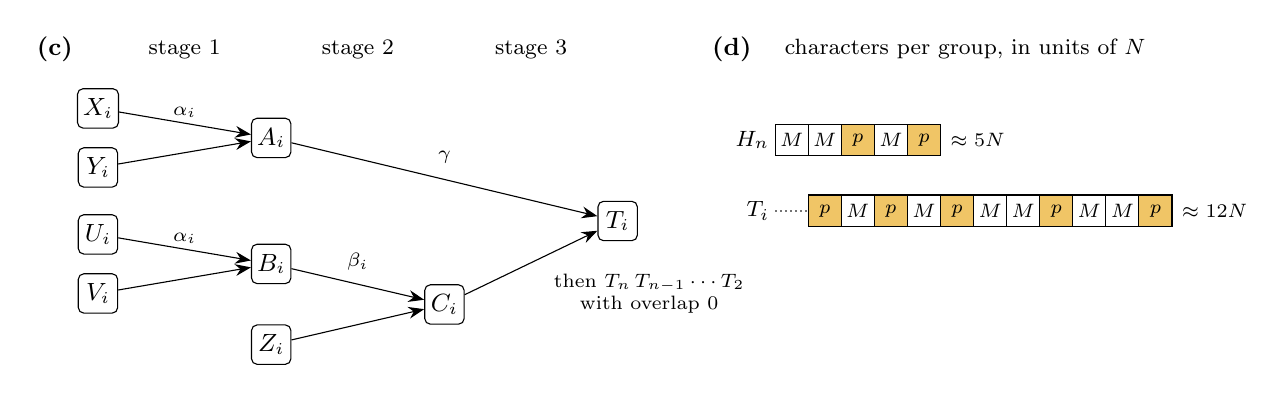
\begin{tikzpicture}[x=1cm,y=1cm]
  % ---- (c) merge order
  \node[panel] at (-0.9,0.75) {(c)};
  \node[font=\footnotesize] at (1.1,0.75) {stage 1};
  \node[font=\footnotesize] at (3.3,0.75) {stage 2};
  \node[font=\footnotesize] at (5.5,0.75) {stage 3};
  \node[vtx] (X) at (0,0) {$X_i$};
  \node[vtx] (Y) at (0,-0.75) {$Y_i$};
  \node[vtx] (U) at (0,-1.6) {$U_i$};
  \node[vtx] (V) at (0,-2.35) {$V_i$};
  \node[vtx] (Z) at (2.2,-3.0) {$Z_i$};
  \node[vtx] (A) at (2.2,-0.375) {$A_i$};
  \node[vtx] (B) at (2.2,-1.975) {$B_i$};
  \node[vtx] (C) at (4.4,-2.49) {$C_i$};
  \node[vtx] (T) at (6.6,-1.43) {$T_i$};
  \draw[->] (X) -- (A); \draw[->] (Y) -- (A);
  \draw[->] (U) -- (B); \draw[->] (V) -- (B);
  \draw[->] (B) -- (C); \draw[->] (Z) -- (C);
  \draw[->] (A) -- (T); \draw[->] (C) -- (T);
  \node[ovl] at (1.1,-0.05) {$\alpha_i$};
  \node[ovl] at (1.1,-1.65) {$\alpha_i$};
  \node[ovl] at (3.3,-1.95) {$\beta_i$};
  \node[ovl] at (4.4,-0.62) {$\gamma$};
  \node[ovl,align=center] at (7.0,-2.35)
    {then $T_n\,T_{n-1}\cdots T_2$\\ with overlap $0$};
  % ---- (d) cost per group
  \begin{scope}[shift={(8.6,0)},x=0.42cm,y=1cm]
    \node[panel] at (-2.2,0.75) {(d)};
    \node[font=\footnotesize,anchor=west] at (0,0.75) {characters per group, in units of $N$};
    \foreach \j in {2,4} \fill[pcol!60] (\j,-0.6) rectangle (\j+1,-0.2);
    \foreach \l [count=\j from 0] in {M,M,p,M,p}{
      \draw (\j,-0.6) rectangle (\j+1,-0.2);
      \node[ovl] at (\j+0.5,-0.4) {$\l$};}
    \node[slabel] at (0,-0.4) {$H_n$};
    \node[ovl,anchor=west] at (5.2,-0.4) {$\approx5N$};
    \draw[densely dotted,thick,black!55] (0,-1.3) -- (1,-1.3);
    \foreach \j in {1,3,5,8,11} \fill[pcol!60] (\j,-1.5) rectangle (\j+1,-1.1);
    \foreach \l [count=\j from 1] in {p,M,p,M,p,M,M,p,M,M,p}{
      \draw (\j,-1.5) rectangle (\j+1,-1.1);
      \node[ovl] at (\j+0.5,-1.3) {$\l$};}
    \node[slabel] at (0,-1.3) {$T_i$};
    \node[ovl,anchor=west] at (12.2,-1.3) {$\approx12N$};
  \end{scope}
\end{tikzpicture}
\caption{The adapted $12/5$ construction. (a)~The gap notation.
(b)~One group $i$ of the short superstring $H_n$ (lengths schematic, private
gaps $p_i$ in orange). The five inputs of group $i$ are windows of the gap
sequence $(M,M,p_i,M,p_i,M,M)$ of $H_n$ (gap positions numbered $1$--$7$
as in Appendix~\ref{app:shibata}), and their zero pads (dotted) fit
into the neighbouring gaps. (c)~The prescribed greedy execution: first
$A_i=X_i\oplus Y_i$ and $B_i=U_i\oplus V_i$ (overlap $\alpha_i$), then
$C_i=B_i\oplus Z_i$ ($\beta_i$), then $T_i=A_i\oplus C_i$ ($\gamma$), each
stage in decreasing order of $i$; the blocks $T_i$ share nothing. (d)~Each
group costs about $5N$ characters in $H_n$ but about $12N$ in greedy's
output (left pad dotted), which gives the ratio $12/5$.}\label{fig:twelve-fifths}
\end{figure}

\begin{theorem}\label{thm:lower-twelve-fifths}
For every $\varepsilon>0$, some $S_n$ admits a valid greedy execution
whose output has length at least $(12/5-\varepsilon)\OPT(S_n)$.
\end{theorem}
\begin{proof}
Construct $H_n$ with left pad $p_n-1$, right pad $N+1$, and gap sequence
\[
 (M,M,p_n,M,p_n)(M,M,p_{n-1},M,p_{n-1})
 \cdots(M,M,p_2,M,p_2)(M,M).
\]
For each $i$, the five input gap sequences are overlapping windows in
$(M,M,p_i,M,p_i,M,M)$. The available zero runs accommodate their pads,
as checked in Appendix~\ref{app:shibata}. Thus $H_n$ is a common
superstring, and
\[
 |H_n|=(3n-1)M+2\sum_{i=2}^np_i+(p_n-1)+(N+1)+1
       =5n^3+O(n^2).
\]

The bad greedy execution first forms
$A_i=X_i\oplus Y_i$ and $B_i=U_i\oplus V_i$ in decreasing order of $i$,
then forms $C_i=B_i\oplus Z_i$ in decreasing order, and finally forms
$T_i=A_i\oplus C_i$. The respective overlap lengths are
\[
 \alpha_i=5N+8n+i+1,\qquad
 \beta_i=4N+8n+i+1,\qquad
 \gamma=2N+2n+1.
\]
Appendix~\ref{app:shibata} proves that every prescribed pair is a current
maximum-overlap pair. The resulting string is
\[
 T_i=[N+n\mid p_i,M,p_i,M,p_i,M,M,p_i,M,M,p_i\mid0].
\]
For $i\ne j$, its overlap with $T_j$ is zero: matching two ones would
require the final gap $p_i$ to equal $p_j$ or $M$, whereas matching just
one would require $N+n$ zeros before the last one of $Z_i$, which has
only $p_i-1<N+n$ zeros. The greedy execution therefore concatenates the
$T_i$, giving
\[
 \GR_n=\sum_{i=2}^n(N+n+1+6M+5p_i)=12n^3+O(n^2).
\]
Since $\OPT(S_n)\le|H_n|$,
\[
 \frac{\GR_n}{\OPT(S_n)}
 \ge\frac{\GR_n}{|H_n|}
 =\frac{12n^3+O(n^2)}{5n^3+O(n^2)}
 \longrightarrow\frac{12}{5}.
\]
Hence the claimed inequality holds for all sufficiently large $n$.
\end{proof}
The construction specifies choices among tied maxima. It proves a lower
bound through one valid execution; $H_n$ is a feasible superstring and is
not asserted to be optimal.

% =====================================================================
\section{Experimental Evaluation}\label{sec:experiments}
% =====================================================================

All code is Python (the standard library, plus numpy for one DP engine),
and every benchmark ran single-process on an idle machine;
Appendix~\ref{app:repro} lists the commands, seeds and hardware.

\subsection{Exact solver: subset dynamic programming}
By Lemma~\ref{lem:perm}, $\OPT=L-\max_\sigma\sum_k\ov(t_k,t_{k+1})$. For
$T\subseteq S$ and $s_i\in T$ let $D(T,i)$ be the largest total overlap of
an ordering of $T$ that ends with $s_i$. Then $D(\{s_i\},i)=0$ and
$D(T\cup\{s_j\},j)=\max_{s_i\in T}\bigl(D(T,i)+\ov(s_i,s_j)\bigr)$ for
$s_j\notin T$, since the gain from appending $s_j$ depends only on the last
string placed. Hence $\OPT=L-\max_iD(S,i)$, and a predecessor table recovers
an optimal order. After an $O(n^2\ell)$ overlap matrix (Knuth--Morris--Pratt,
$\ell$ the maximum length) this takes $O(n^22^n)$ time and $O(n2^n)$ space.
Our pure-Python engine needs 11.5\,s at $n=20$; a numpy engine needs 0.68\,s
at $n=20$ and 15\,s at $n=24$, but its estimated 5.6\,GB at $n=25$ exceeded
our 4\,GB budget (Appendix~\ref{app:extra}). Memory is thus the binding
constraint, and our benchmarks stop at $n=20$. Appendix~\ref{app:validation}
describes independent checks of both engines.

\subsection{Greedy implementation and tie-breaking rules}
Our greedy follows Algorithm~\ref{alg:greedy}: each step scans all ordered
pairs of current strings, and by Lemma~\ref{lem:greedy-graph} the overlaps
of $s\oplus t$ are copied from $s$ (incoming) and $t$ (outgoing). Every
merge is logged and replayed by an independent validator that recomputes
all overlaps naively. Retained strings get IDs in lexicographic order, and
the $t$-th merged string gets ID $n+t$. Ties are broken by
\texttt{lowest\_id} or \texttt{highest\_id} (smallest or largest ID pair; the
latter prefers recently merged strings), by \texttt{lex\_merged} (the pair
whose merged string is lexicographically smallest), or by \texttt{random}
(uniform among the tied pairs, seeded separately from the instance). Each
instance gets one run per deterministic rule and ten \texttt{random} runs,
13 runs on the same input. A \emph{prescribed} merge sequence, such as a
published bad execution, is replayed through the same validator.

\subsection{Instance families and metrics}
The benchmark has 4{,}935 instances with $n\in\{5,8,10,12,15,18,20\}$
strings \emph{after} preprocessing (strings are drawn until exactly $n$
survive).
(A)~\emph{Random strings} (1{,}260) over a binary or four-letter alphabet,
of length 3--8, 8--14 or exactly 7.
(B)~\emph{Fragments} (2{,}100) of a random binary or four-letter source, of
length 4--8 or 8--14 at coverage 0.5, 1 or 2.
(C)~\emph{Repetitive fragments} (1{,}575) of length 6--12 from a four-letter
source of mutated copies of one motif (length 6, 12 or 24; mutation rate
0.05, 0.10 or 0.25).
Preprocessing removed on average 10\%, 29\% and 36\% of the drawn strings in
(A), (B) and (C).
(D)~\emph{Known and discovered instances} (18), reported separately: cases
such as \str{ATT}, \str{TTA}, \str{TAC}, the family $S_k$ of
Section~\ref{sec:lower-two} for $k\le6$, and seven instances from a search
for bad ratios (Appendix~\ref{app:extra}).
(E)~\emph{Sequencing reads}: 76\,bp Illumina reads of the phiX174 phage
(ENA run ERR098007), kept in the reported orientation and unfiltered. For
each $n\in\{5,8,10,12,15,18\}$ we drew 30 \emph{unconditioned} subsets from all
23{,}118 eligible reads, errors included, and 30 reference-assisted
\emph{local} subsets of reads that match the reference exactly and lie within
a random 250\,bp window.
(F)~\emph{Shibata's construction}~\cite{Shi26}
(Section~\ref{sec:shibata-exp}).

We report $\GR/\OPT$, the optimality rate (fraction of instances with
$\GR=\OPT$) and the compression ratio, which is defined throughout because
$L>\OPT$ in every benchmark instance. The \texttt{random} runs are averaged per instance
before any statistic across instances. An instance is
\emph{tie-sensitive} if its 13 runs give more than one length; the worst of
them only bounds the worst valid execution from below.

\subsection{Results}

\begin{table}[h]\centering\small
\caption{Greedy against exact $\OPT$ on the benchmark ($n=5,\dots,20$) and
on phiX174 reads ($n=5,\dots,18$). The optimality rate and the mean and
95th percentile of $\GR/\OPT$ refer to \texttt{lowest\_id}; the maximum of
$\GR/\OPT$ is over all 13 runs; ``tie-sens.'' is the fraction of
tie-sensitive instances; the last column is the optimality rate of the best
and of the worst of the 13 runs.}\label{tab:synthetic}
\begin{tabular}{lrcccccc}
\toprule
Family & Inst. & Opt.\ rate & Mean & 95th pct. & Max & Tie-sens. & Best / worst\\
\midrule
Random, binary         & 630     & 0.62 & 1.014 & 1.060 & 1.222 & 0.67 & 0.89 / 0.29\\
Random, four-letter    & 630     & 0.80 & 1.003 & 1.021 & 1.067 & 0.55 & 0.99 / 0.44\\
Fragments, binary      & 1{,}050 & 0.63 & 1.015 & 1.069 & 1.583 & 0.57 & 0.88 / 0.38\\
Fragments, four-letter & 1{,}050 & 0.82 & 1.004 & 1.023 & 1.200 & 0.39 & 0.98 / 0.59\\
Repetitive, motif 6    & 525     & 0.56 & 1.025 & 1.109 & 1.435 & 0.59 & 0.79 / 0.32\\
Repetitive, motif 12   & 525     & 0.63 & 1.019 & 1.100 & 1.320 & 0.52 & 0.81 / 0.39\\
Repetitive, motif 24   & 525     & 0.75 & 1.007 & 1.036 & 1.171 & 0.44 & 0.91 / 0.50\\
\midrule
All benchmark          & 4{,}935 & 0.70 & 1.012 & 1.062 & 1.583 & 0.52 & 0.90 / 0.43\\
\midrule
phiX174, unconditioned & 180     & 0.81 & 1.000 & 1.002 & 1.005 & 0.46 & 0.95 / 0.53\\
phiX174, local         & 180     & 1.00 & 1.000 & 1.000 & 1.000 & 0.00 & 1.00 / 1.00\\
\bottomrule
\end{tabular}
\end{table}

\paragraph{Typical instances.} Table~\ref{tab:synthetic} shows greedy nearly
optimal on typical inputs: under \texttt{lowest\_id} the median ratio is
$1.000$ for every family and size except repetitive inputs at $n=20$
($1.008$). The optimality rate still
falls with $n$, from $0.84$--$0.92$ at $n=5$ to $0.49$--$0.63$ at $n=20$
(Appendix~\ref{app:extra}). Low-entropy inputs are harder: a binary alphabet
lowers the rate from about $0.8$ to $0.6$, and short motifs with few
mutations are worst. The traces show one recurring mechanism: a
maximum-overlap merge joins two strings that each had a good partner elsewhere, stranding a
string that can later be attached only with overlap~$0$. In the worst
benchmark instance (binary fragments, $n=5$), \texttt{lowest\_id} merges
$\str{AB}^7$ with $\str{B}^7\str{A}$ and strands $\str{B}^8$, as in $S_h$ of
Section~\ref{sec:compression}, giving length 19 against $\OPT=12$, while
\texttt{highest\_id} is optimal.

\paragraph{Tie-breaking.} The tie-sensitive fraction grows from
$0.15$--$0.28$ at $n=5$ to $0.68$--$0.73$ at $n=20$. The spread in length is
small (about $2\%$ of $\OPT$ on average, at most 11 characters) but decides
optimality: at $n=20$ the best run is optimal on $0.80$--$0.90$ of
instances, \texttt{lowest\_id} on $0.49$--$0.63$ and the worst run on
$0.20$--$0.30$ (Figure~\ref{fig:ties}, Appendix~\ref{app:extra}). No deterministic rule is
consistently better. On $S_k$ the bad merge is the unique maximum, so every
rule gives $(4k+2)/(2k+4)$, reaching $1.625$ at $k=6$. The discovered
instances are instead tie-driven, optimal under one rule and of ratio
$1.43$--$1.57$ under another; four are exactly $S_h$ of
Section~\ref{sec:compression} with $\str{c}=\str{a}$, which leaves its
argument unchanged.

\paragraph{Compression.} All 64{,}155 benchmark runs, 4{,}680 phiX174 runs
and family~(D) runs satisfy $L-\GR\ge\frac12(L-\OPT)$. The minimum
compression ratio was $0.500$ for random strings, $0.667$ for fragments and
unconditioned reads, and $0.739$ for repetitive inputs; 68\% of benchmark
runs had ratio exactly~1. The bound was attained only by six discovered
instances ($S_h$ and close variants) and by two random instances with tiny
optimal compression ($L-\OPT=2$ and $4$). The constant $\frac12$ of
Theorem~\ref{thm:half} is thus tight even on tiny inputs, though the 1st
percentile is $0.85$--$0.90$ in every benchmark family.

\paragraph{Sequencing reads.} On local reads greedy was optimal in all 180
subsets under every rule and seed, since exact reads from a short window
form a simple path with long, mostly unique overlaps. Unconditioned reads
overlap mostly by a few characters by chance; greedy missed $\OPT$ on 19\%
of them, yet $\GR/\OPT\le1.005$ because $\OPT$ is in the hundreds. This
concerns superstrings of the supplied reads, not genome assembly: about half
of the reads do not occur exactly in the reference, and 17\% of those that
do come from the reverse strand.

\subsection{Reproducing Shibata's construction}\label{sec:shibata-exp}
Shibata's $S_{k,t}$~\cite{Shi26}, for even $k$ and $s=k/2$, consists of all
length-$k$ cyclic substrings of $3t$ periodic words over
$\{\str{x},\str{y},\str{a},\str{b}_1,\dots,\str{b}_t\}$, $n=t(2k+2)$
strings in total. A prescribed valid execution has length $t(9s+1)+1$,
whereas $\OPT=t(4s+2)+k-1$, so the ratio tends to $(9k+2)/(4k+4)$ as
$t\to\infty$ and to $9/4$ as $k\to\infty$. We replayed this execution for 15
pairs with $k\in\{10,12,16,20\}$ and $t\le16$: every merge attained the
current maximum, and every output had the predicted length. We certified
$\OPT$ independently: $n$ distinct length-$k$ strings need $n$ distinct
windows, so $\OPT\ge n+k-1$, and an Eulerian circuit in the order-$(k-1)$
de~Bruijn graph of the inputs gives a superstring of that length. The DP
confirms $\OPT=31$ at $(k,t)=(10,1)$. Figure~\ref{fig:shibata} shows the
three periodic words of one group.

\begin{figure}[htb]\centering
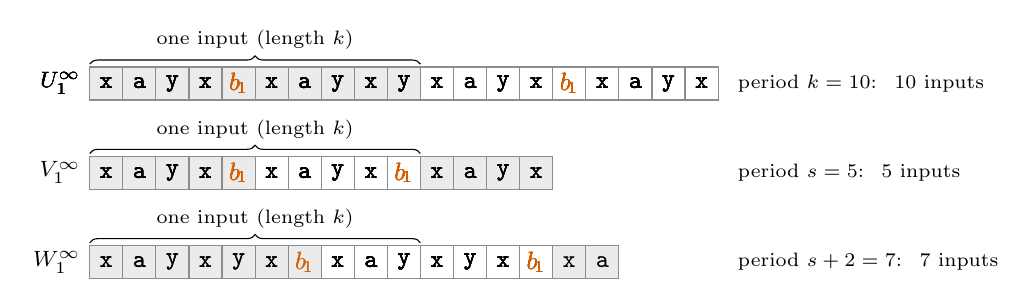
\begin{tikzpicture}[x=0.42cm,y=0.42cm]
  \def\B{{\color{gcol}$b_{\!1}$}}
  \foreach \y/\a/\b in {0/0/9,-2.7/0/4,-2.7/10/13,-5.4/0/6,-5.4/14/15}
    \shadecells[black!8]{\a}{\b}{\y}
  \cellrow{0}{0}{x,a,y,x,\B,x,a,y,x,y,x,a,y,x,\B,x,a,y,x}
  \cellrow{0}{-2.7}{x,a,y,x,\B,x,a,y,x,\B,x,a,y,x}
  \cellrow{0}{-5.4}{x,a,y,x,y,x,\B,x,a,y,x,y,x,\B,x,a}
  \node[slabel] at (-0.6,0) {$U_1^\infty$};
  \node[slabel] at (-0.6,-2.7) {$V_1^\infty$};
  \node[slabel] at (-0.6,-5.4) {$W_1^\infty$};
  \foreach \y in {0,-2.7,-5.4}
    \draw[brc] (-0.5,\y+0.5) -- node[above=5pt,ovl]{one input (length $k$)} (9.5,\y+0.5);
  \node[ovl,anchor=west] at (19,0) {period $k=10$: \ $10$ inputs};
  \node[ovl,anchor=west] at (19,-2.7) {period $s=5$: \ $5$ inputs};
  \node[ovl,anchor=west] at (19,-5.4) {period $s+2=7$: \ $7$ inputs};
\end{tikzpicture}
\caption{Shibata's $S_{k,t}$ for $(k,t)=(10,1)$, $s=k/2$. Group $i$ uses
the words $U_i=\str{xa}X_{s-3}b_i\str{xa}X_{s-3}\str{y}$,
$V_i=\str{xa}X_{s-3}b_i$ and $W_i=\str{xa}X_{s-1}b_i$, where $X_m$ is the
alternating word in \str{x},\str{y} of length $m$ ending in \str{x}, and
its inputs are all length-$k$ windows of $U_i^\infty$, $V_i^\infty$ and
$W_i^\infty$, one per starting position in a period (one period shaded):
$k+s+(s+2)=2k+2$ strings per group.}\label{fig:shibata}
\end{figure}

\begin{table}[h]\centering\small
\caption{Shibata's $S_{k,t}$ with certified $\OPT$. ``Prescribed'' is the
paper's bad execution, checked step by step; the last four columns give the
lengths from our rules on the same input (\texttt{random}: range over 50
seeds; not run for $n>200$).}\label{tab:shibata}
\setlength{\tabcolsep}{4pt}
\begin{tabular}{rrrrrcrrrc}
\toprule
$k$ & $t$ & $n$ & $\OPT$ & Prescribed & $\GR/\OPT$ & \texttt{lowest\_id} & \texttt{highest\_id} & \texttt{lex\_merged} & \texttt{random}\\
\midrule
10 & 1  & 22  & 31  & 47      & 1.516 & 38  & 42  & 43  & 31--44\\
10 & 4  & 88  & 97  & 185     & 1.907 & 149 & 168 & 172 & 110--154\\
10 & 9  & 198 & 207 & 415     & 2.005 & 334 & 378 & 387 & 245--322\\
10 & 16 & 352 & 361 & 737     & 2.042 & --  & --  & --  & --\\
16 & 16 & 544 & 559 & 1{,}169 & 2.091 & --  & --  & --  & --\\
20 & 16 & 672 & 691 & 1{,}457 & 2.109 & --  & --  & --  & --\\
\bottomrule
\end{tabular}
\end{table}

Table~\ref{tab:shibata} shows the prescribed execution exceeding $2\,\OPT$
from $(k,t)=(10,9)$ and reaching $2.109$ at $(20,16)$, a machine-checked
confirmation that the historical conjecture fails on these inputs; the
limit for $k=20$ is $2.167$. The bad execution needs specific ties: at
$(10,9)$ our deterministic rules gave ratios $1.61$--$1.87$ and 50
random-tie runs $1.18$--$1.56$, and the rules' ratios grow with $t$
(\texttt{lex\_merged} rises from $1.39$ at $t=1$). Even above $2\,\OPT$ its
compression ratio is $0.88$--$0.94$, showing how far apart the two
guarantees are.

\subsection{Discussion}
Outside constructed and searched-for instances the largest ratio we
observed was $1.583$, far below $12/5\le\rho\le3$: bad cases need structure
and, for Shibata's instances, tie choices our rules did not make
(Nikolaev's equivalence~\cite{Nik21} concerns perturbed inputs, not a given
one). The 2-approximation of~\cite{OAI26}, which we also implemented,
averaged $1.27\,\OPT$ on families (A)--(D) (Appendix~\ref{app:extra}).
\emph{Threats to validity.} Exact optima cover only $n\le20$, the families
are our own design, 13 runs sample the tie choices without bounding them,
and timings come from one machine under Python. The Shibata reproduction
covers only the listed parameters and our reading of the preprint.

% =====================================================================
\section{Conclusion}\label{sec:conclusion}
% =====================================================================

\subsection{Summary}
We proved that every valid greedy execution achieves at least half the
optimal compression using two matchings and a Monge inequality. For length,
we proved the cycle-cover inequality behind the factor-$3$ guarantee and
simplified the $12/5$ lower-bound construction to one parameter. Thus the
compression factor $1/2$ is tight, while greedy's worst-case length ratio
lies between $12/5$ and $3$.

On 4{,}935 benchmark instances with up to 20 strings, greedy averaged
within $1.2\%$ of optimal and its worst ratio was $1.583$. It was optimal on
every error-free local set of phiX174 reads and within $0.5\%$ on
unconditioned reads. Its optimality rate nevertheless fell from
$0.84$--$0.92$ at $n=5$ to $0.49$--$0.63$ at $n=20$, and tie-breaking
decided much of this: at $n=20$ the best of our 13 runs was optimal on
80--90\% of instances and the worst on only 20--30\%. Every run respected
the half-compression bound, which was attained exactly only on tiny
instances, including members of the tightness family $S_h$. Shibata's
construction, replayed with certified optima, gave ratios up to $2.109$, but
only under prescribed ties; our own rules gave at most $1.87$ on the
instances with up to 200 strings where we ran them. These results separate
typical behaviour from the worst case. Sequencing errors and mixed strands
also limit the practical applicability of plain SCS.

\subsection{State of the art and beyond our scope}
Closing the gap $12/5\le\rho\le3$ remains open. For general SCS,
approximation factors improved from $2\frac{11}{23}$~\cite{Muc13} through
$2.475$~\cite{EMV22} and $2.466$~\cite{EMV23} to $7/3$~\cite{CKMS26};
approximation below $333/332$ is NP-hard~\cite{KS13}.
A 2026 OpenAI preprint~\cite{OAI26} gives a deterministic $2$-approximation
in time polynomial in the full encoded input size. Its algorithm differs
from maximum-overlap greedy, the focus of this report, so we do not analyse
it; in our experiments it was far longer than greedy on typical inputs
(Appendix~\ref{app:extra}). Further directions include
smoothed or average-case analysis and assembly models with reverse
complements or sequencing errors.

\label{endofbody}   % <-- main body must end on or before page 10



% =====================================================================
\section{AI disclosure}\label{sec:ai-use}
% =====================================================================

In preparing this project, we used Claude (Anthropic Claude Opus 5.5) in the following ways.
Claude was used as an assistant to research the topic, to generate the LaTeX for various formulae and to proofread the text for accuracy.
The code for instance generation, the subset DP and our greedy implementation
was also generated with Claude, with human proofreading of its logic and of the interpretation of the data it generated.
Claude also drafted the experimental section (Section~\ref{sec:experiments}), the experimental
appendices (Appendices~\ref{app:validation}--\ref{app:repro}) and the experimental parts of the
abstract and conclusion from our repository's results. It independently re-verified those results
by re-implementing greedy and the exact solver, re-running the experiments from their seeds and
checking the constructions of Sections~\ref{sec:compression} and~\ref{sec:worstcase} computationally.

GPT (OpenAI) was also used to help the authors understand the proofs in the
original papers, draft detailed proofs, and carry out a final check of the
manuscript, including its mathematical arguments, references, and presentation.

We have checked all AI-assisted content and take full responsibility for the correctness and presentation of the final submission.


% =====================================================================
%  References
% =====================================================================
\newpage
{\small
\begin{thebibliography}{99}\setlength{\itemsep}{0pt}
\bibitem{BJLTY94} A.~Blum, T.~Jiang, M.~Li, J.~Tromp and M.~Yannakakis.
  Linear approximation of shortest superstrings.
  \emph{Journal of the ACM} 41(4):630--647, 1994.
  \url{https://doi.org/10.1145/179812.179818}

\bibitem{CKMS26} N.~Chukhin, A.~S.~Kulikov, I.~Mihajlin and A.~Smal.
  A tight cycle-cover inequality for shortest common superstring.
  arXiv:2609.27921v2 / ECCC TR26-157, 2026. Preprint.
  \url{https://arxiv.org/abs/2609.27921v2}

\bibitem{GSC26} N.~Chukhin, R.~Gajjala, J.~Harviainen, A.~S.~Kulikov,
  I.~Mihajlin, H.~Shibata and A.~V.~Smal.
  The greedy superstring conjecture is false.
  November 2026. Preprint.
  \url{https://arxiv.org/abs/2609.01365v2}

\bibitem{EMV22} M.~Englert, N.~Matsakis and P.~Vesel\'y.
  Improved approximation guarantees for shortest superstrings using cycle
  classification by overlap to length ratios.
  In \emph{Proc.\ STOC 2022}, pp.~317--330, ACM, 2022.
  \url{https://doi.org/10.1145/3519935.3520001}

\bibitem{EMV23} M.~Englert, N.~Matsakis and P.~Vesel\'y.
  Approximation guarantees for shortest superstrings: simpler and better.
  In \emph{Proc.\ ISAAC 2023}, LIPIcs 283, pp.~29:1--29:17, 2023.
  \url{https://doi.org/10.4230/LIPIcs.ISAAC.2023.29}

\bibitem{FKRRW16} G.~Fici, T.~Kociumaka, J.~Radoszewski, W.~Rytter and
  T.~Wale\'n. On the greedy algorithm for the shortest common superstring
  problem with reversals. \emph{Information Processing Letters}
  116(3):245--251, 2016.
  \url{https://doi.org/10.1016/j.ipl.2015.11.015}

\bibitem{GMS80} J.~Gallant, D.~Maier and J.~A.~Storer.
  On finding minimal length superstrings.
  \emph{Journal of Computer and System Sciences} 20(1):50--58, 1980.
  \url{https://doi.org/10.1016/0022-0000(80)90004-5}

\bibitem{KN24} P.~E.~Kalugin and M.~S.~Nikolaev.
  The greedy algorithm for the shortest common superstring problem is a
  $\tfrac12$-approximation in terms of compression: a simple proof.
  In \emph{Proc.\ SOSA 2024}, pp.~97--99, SIAM, 2024.
  \url{https://doi.org/10.1137/1.9781611977936.9}

\bibitem{KS05} H.~Kaplan and N.~Shafrir.
  The greedy algorithm for shortest superstrings.
  \emph{Information Processing Letters} 93(1):13--17, 2005.
  \url{https://doi.org/10.1016/j.ipl.2004.09.012}

\bibitem{KS13} M.~Karpinski and R.~Schmied.
  Improved inapproximability results for the shortest superstring and
  related problems. In \emph{Proc.\ CATS 2013}, pp.~27--36, 2013.
  Preprint: \url{https://theoryx.informatik.uni-bonn.de/ftp/reports/cs-reports/2012/85331-CS.pdf}

\bibitem{Muc13} M.~Mucha.
  Lyndon words and short superstrings.
  In \emph{Proc.\ SODA 2013}, pp.~958--972, SIAM, 2013.
  \url{https://doi.org/10.1137/1.9781611973105.69}

\bibitem{Nik21} M.~S.~Nikolaev.
  All instantiations of the greedy algorithm for the shortest common
  superstring problem are equivalent.
  In \emph{Proc.\ SPIRE 2021}, pp.~61--67, 2021.
  \url{https://arxiv.org/abs/2102.05579}

\bibitem{OAI26} OpenAI.
  A polynomial-time 2-approximation for shortest common superstring.
  Preprint, 2026.
  \href{https://github.com/openai/math/blob/main/preprints/A-Polynomial-Time-2-Approximation-for-Shortest-Common-Superstring-September-24-2026/paper.pdf}{\nolinkurl{github.com/openai/math}} (result~128).

\bibitem{Shi26} H.~Shibata.
  Disproving the greedy superstring conjecture.
  arXiv:2609.01365v1, 2026. Preprint.
  \url{https://arxiv.org/abs/2609.01365v1}

\bibitem{TU88} J.~Tarhio and E.~Ukkonen.
  A greedy approximation algorithm for constructing shortest common
  superstrings. \emph{Theoretical Computer Science} 57(1):131--145, 1988.
  \url{https://doi.org/10.1016/0304-3975(88)90167-3}

\bibitem{Tur89} J.~S.~Turner.
  Approximation algorithms for the shortest common superstring problem.
  \emph{Information and Computation} 83(1):1--20, 1989.
  \url{https://doi.org/10.1016/0890-5401(89)90044-8}
\end{thebibliography}
}



% ======== We can see later if we need these sections or they fit into the  main body ============

\clearpage
\appendix
\section*{Appendix}\addcontentsline{toc}{section}{Appendix}
\renewcommand{\thesubsection}{\Alph{subsection}}

\subsection{Details of the adapted \texorpdfstring{$12/5$}{12/5} construction}\label{app:shibata}

We use the notation and family of Section~\ref{sec:lower-twelve-fifths}.
The following checks justify the adjusted gap and padding constants in
our single-parameter adaptation of Chukhin et al.~\cite{GSC26}.

\paragraph{Computing overlaps from gaps.}
Let $s=[a\mid u_1,\ldots,u_k\mid b]$ and
$t=[c\mid v_1,\ldots,v_\ell\mid d]$ be substring-free strings.
An overlap containing $q+1$ ones must match the last $q$ gaps of $s$
with the first $q$ gaps of $t$. Its form and length are
\[
 [c\mid v_1,\ldots,v_q\mid b],
 \qquad c+b+1+\sum_{h=1}^qv_h.
\]
The left pad fits precisely when $c<u_{k-q}$ if $q<k$, or $c\le a$ if
$q=k$. The right pad fits when $b<v_{q+1}$ if $q<\ell$, or $b\le d$
if $q=\ell$. These conditions also apply when $q=0$, with no shared
gaps. An overlap containing no ones consists of $\min\{b,c\}$ zeros.
Maximizing over these possibilities computes $\ov(s,t)$.

\paragraph{Substring-freeness and the short superstring.}
Every input with index $i$ contains a private gap $p_i$, so an input
cannot be contained in one with another index. Within a group, the four
five-one strings have different complete gap sequences. The four-one
string $Z_i$ has gap sequence $(M,M,p_i)$, which occurs only at the start
of $U_i$ among those four strings. Its left pad is $p_i-1>N$, whereas
$U_i$ has left pad $N$, preventing containment. Thus $S_n$ is
substring-free.

In $H_n$, number the gaps of the local segment
$(M,M,p_i,M,p_i,M,M)$ from $1$ to $7$. The input gap sequences occupy
the following windows:
\[
 \begin{array}{c|ccccc}
 \text{Input}&Z_i&U_i&Y_i&X_i&V_i\\ \hline
 \text{Gap positions}&1\text{--}3&1\text{--}4&
 2\text{--}5&3\text{--}6&4\text{--}7
 \end{array}
\]
The longer pads of $X_i,Y_i$ fit into the adjacent common gaps because
$M-1\ge N+2n$. The pads of $U_i$ also fit, since every private gap has
at least $N+1$ zeros. Before $Z_i$, the available zero run has length
$p_{i+1}-1\ge p_i-1$ if $i<n$; the left pad of $H_n$ handles $i=n$.
After $V_i$, the available run has length $p_{i-1}-1\ge N+1$ if $i>2$;
the right pad of $H_n$ handles $i=2$. The remaining pads are no longer
than these runs. This proves that $H_n$ contains every input.

\paragraph{Intermediate strings and prescribed overlaps.}
The overlap rule gives
\[
\begin{aligned}
 A_i&=[N+n\mid p_i,M,p_i,M,p_i\mid N+2n],\\
 B_i&=[N\mid M,M,p_i,M,M\mid N+1],\\
 C_i&=[N\mid M,M,p_i,M,M,p_i\mid0].
\end{aligned}
\]
The first two merges share $(M,p_i,M)$ with pads $N,N$ and have overlap
$\alpha_i=2N+2M+p_i+1$. The merge $B_i\to Z_i$ shares $(M,M)$ with
pads $p_i-1,N+1$ and has overlap
$\beta_i=N+2M+p_i+1$. The merge $A_i\to C_i$ shares only one one,
with pads $N,N+2n$, and has overlap $\gamma=2N+2n+1$.
In the following checks, Lemma~\ref{lem:greedy-graph} lets us compute
overlaps through the original first and last inputs after each valid
merge.

\paragraph{Validity of the first stage.}
Put $D=3N+7n+1$ and $\lambda=4N+8n+2$.
An overlap of two inputs sharing at most one gap has length at most $D$.
Two shared gaps involving a private gap have total gap length at most
$M+p_n$, so the overlap length is at most $4N+8n+1$.
Two shared gaps $(M,M)$ can occur only from $V_i$ to $U_j$ or $Z_j$:
the former overlap is $\lambda$, and the latter is at most $\beta_j$.
No distinct inputs share four gaps. The possibilities sharing three
gaps are exactly
\[
\begin{array}{c|c}
 \text{Ordered pair}&\text{Overlap length}\\ \hline
 (X_i,Y_i),(X_i,V_i),(U_i,Y_i),(U_i,V_i)&\alpha_i\\
 (Y_i,X_i)&5N+7n+2i+1=\alpha_i-(n-i)\\
 (Z_i,U_i)&\beta_i
\end{array}
\]
Consequently, every input overlap larger than $\beta_n$ is one of the
first five types in this table, has a common index, and is at most
$\alpha_i$. Moreover,
\[
 \alpha_2-\beta_n=N-n+2>0.
\]
After processing indices greater than $i$, the current strings are
$A_j,B_j,Z_j$ for $j>i$ and the five original inputs for $j\le i$.
For a processed index, none of those five large pair types can connect
two distinct current strings: their endpoints have been consumed into
$A_j,B_j$, or the pair would close the same current string. All overlaps
involving processed groups are therefore at most $\beta_n$.
The largest remaining overlap is $\alpha_i$, attained by $X_i\to Y_i$
and, after that merge, still by $U_i\to V_i$. Induction proves the
validity of the first stage.

\paragraph{Validity of the second stage.}
The current strings initially are $A_i,B_i,Z_i$. After some prescribed
merges, there are also completed strings $C_i$. Among distinct current
strings, the only overlaps larger than $\lambda$ can be
\[
 B_i\to Z_j\quad(j\le i),\qquad Z_i\to B_i,
\]
with lengths $\beta_j$ and $\beta_i$, respectively.
Indeed, for $B_i\to Z_j$ the two shared gaps $(M,M)$ fit precisely when
$p_j-1<p_i$, or $j\le i$; the other pad fits because $N+1<p_j$.
If $j>i$, at most one gap is shared. The overlap $Z_i\to B_i$
shares $(M,M,p_i)$ and has length $\beta_i$.
Pairs $B_i\to B_j$ and $B_i\to C_j$, when present, have overlap
$\lambda$. All remaining pairs share at most one gap and have overlap
at most $D<\lambda$, since a same-index $A_i\to A_i$ or
$C_i\to C_i$ is not a pair of distinct current strings.

If $k$ is the largest unprocessed index, the maximum is therefore
$\beta_k>\lambda$, attained by $B_k\to Z_k$. Creating $C_k$ removes
both sources of a large overlap with index $k$, and the same argument
applies to $k-1$. Thus the second stage is valid in decreasing index order.

\paragraph{Validity of the third stage and final concatenation.}
When only $A_i,C_i$ remain, direct gap matching gives
\[
\begin{aligned}
 \ov(A_i,A_j)&=N+n &&(i\ne j),\\
 \ov(C_i,C_j)&=N+1 &&(i\ne j),\\
 \ov(A_i,C_j)&=\gamma &&(\text{all }i,j),\\
 \ov(C_i,A_j)&=
 \begin{cases}
 2N+n+i+1,&i=j,\\
 0,&i\ne j.
 \end{cases}
\end{aligned}
\]
Every value is at most $\gamma$, since $i\le n$.
Hence $A_i\to C_i$ is a maximum-overlap choice. A resulting $T_i$
starts with $X_i$ and ends with $Z_i$; the displayed bounds and
Lemma~\ref{lem:greedy-graph} show that its overlaps with remaining
strings are also at most $\gamma$. Thus the other prescribed pairs can
still be chosen.

For $i\ne j$, $\ov(T_i,T_j)=\ov(Z_i,X_j)=0$. An overlap with at least
two ones would require $p_i$ to be a gap of $X_j$, but its gaps are
$p_j,M$. An overlap with just one one would require $N+n$ zeros before
the final one of $Z_i$, exceeding $p_i-1$. Finally, $Z_i$ ends with a
one, so there is no nonempty all-zero overlap. Concatenation of the
$T_i$ is therefore the final greedy stage.

For reference, the exact lengths are
\[
 |H_n|=5n^3+12n^2-2n-1,\qquad
 \GR_n=12n^3+\frac{31n^2-43n-12}{2}.
\]
Their quotient tends to $12/5$. This is the computable lower bound
$\GR_n/|H_n|$ on $\GR_n/\OPT(S_n)$, not a claim that $H_n$ is optimal.

\subsection{Details of the upper bound of three}\label{app:upper}

We justify the classical cycle-word properties used in
Section~\ref{sec:upper-three}, then outline the transfer from cycle covers
to the original greedy algorithm. The counting lemma and the inequality
$O-W\le\OPT$ are already proved in the main text. The exchange and
charging arguments in the transfer are invoked from Blum et
al.~\cite[Section~5]{BJLTY94}.

\paragraph{A periodic placement observation.}
Suppose every string of a nonempty substring-free set $A$ occurs in
$q^\infty$, where $q$ is nonempty. Choose one occurrence of each string
and reduce its starting position modulo $p=|q|$. These residues are
distinct: two strings starting at the same residue would be prefixes of
the same infinite word, so one would contain the other. Order the strings
by their residues $0\le a_1<\cdots<a_k<p$, and put $a_{k+1}=a_1+p$ and
$s_{k+1}=s_1$. The next occurrence of $s_{i+1}$ starts
$d_i=a_{i+1}-a_i>0$ positions after $s_i$.

If $d_i\ge|s_i|$, then $\operatorname{pref}(s_i,s_{i+1})\le d_i$
immediately. Otherwise their occurrences overlap in $|s_i|-d_i$
characters. This is a proper suffix of $s_i$ and a proper prefix of
$s_{i+1}$; the latter follows from substring-freeness (and is immediate
when $k=1$). Thus the maximum overlap gives
$\operatorname{pref}(s_i,s_{i+1})\le d_i$ in this case too. Consequently,
these strings admit a cycle with total prefix cost
\[
 \sum_{i=1}^k\operatorname{pref}(s_i,s_{i+1})
 \le\sum_{i=1}^kd_i=p.
\]
The observation includes a one-vertex cycle, using the proper
self-overlap from Section~\ref{sec:prelim}.

\paragraph{Primitive and distinct cycle words.}
Unfolding the overlaps around a cycle $C$ places every input on $C$
inside $\tau(C)^\infty$, as in the periodic unfolding used
for~\eqref{eq:upper-forced-windows}. If
$\tau(C)=q^h$ for some $h\ge2$, the placement observation gives a cycle
through the same inputs with total prefix cost at most
$|q|<|\tau(C)|=w(C)$. Replacing $C$ by that cycle contradicts the
optimality of $\mathcal C$. Hence every $\tau(C)$ is primitive.

If two distinct cycles have cycle words equivalent up to rotation, their
words have a common length $p$ and all their inputs occur in one common
periodic word. Applying the observation to the union of their inputs
replaces two cycles of total cost $2p$ by one of cost at most $p$, again
a contradiction. Thus their rotation classes are distinct. These are
the classical properties cited in~\cite[Lemma~2.5]{Muc13}.

Each cycle therefore has a distinct Lyndon representative $z_C$ with
$|z_C|=w(C)$. For completeness, a Lyndon word $z$ has no period
$d<|z|$: such a period would make its suffix of length $|z|-d$ equal to
a proper prefix, and hence lexicographically smaller than $z$, whereas
a Lyndon word is strictly smaller than each proper nonempty suffix.
This verifies the properties required by
Lemma~\ref{lem:upper-periodic-count}.

\paragraph{The subset associated with a greedy execution.}
Fix a total order of all overlap edges, including self-loops, compatible
with non-increasing overlap and with the chosen greedy tie-breaking.
View greedy as scanning this order. An edge may be rejected because
it conflicts with an already selected incoming or outgoing edge, or
because it would close a cycle. Call edges rejected solely for the
second reason \emph{bad back edges}.
At least one exists: the edge from the last input of the final greedy
path to its first has no degree conflict, so it must be rejected for
closing a cycle.

Number the inputs in their final greedy order. Each bad back edge
$j\to i$ spans an interval $[i,j]$ whose internal path edges have
already been selected. Blum et al.~\cite[Lemma~13]{BJLTY94} show that
these intervals are nested or disjoint. The minimal, innermost intervals
are called \emph{culprits}; let $U\subseteq S$ consist of their inputs.
Adding each culprit's back edge to its internal path gives an optimal
cycle cover $\mathcal C_U$ of $U$~\cite[Lemma~15]{BJLTY94}.
Each closing edge was considered after the internal path edges, so its
overlap is minimum on its cycle. Thus the quantities $W_U,O_U$ agree
with the definitions in Section~\ref{sec:upper-three}
(Figure~\ref{fig:culprits}).

\begin{figure}[htb]\centering
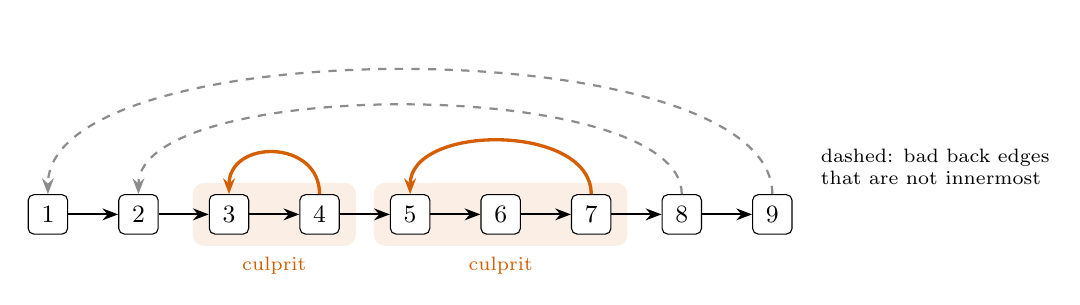
\begin{tikzpicture}[x=1.15cm,y=1cm]
  \fill[gcol!10,rounded corners=4pt] (2.6,-0.4) rectangle (4.4,0.4);
  \fill[gcol!10,rounded corners=4pt] (4.6,-0.4) rectangle (7.4,0.4);
  \foreach \i in {1,...,9} \node[vtx] (v\i) at (\i,0) {$\i$};
  \foreach \i [evaluate=\i as \j using int(\i+1)] in {1,...,8}
    \draw[->,thick] (v\i) -- (v\j);
  \draw[->,thick,black!45,dashed] (v9.north) .. controls +(0,2.1) and +(0,2.1) .. (v1.north);
  \draw[->,thick,black!45,dashed] (v8.north) .. controls +(0,1.5) and +(0,1.5) .. (v2.north);
  \draw[->,very thick,gcol] (v4.north) .. controls +(0,0.7) and +(0,0.7) .. (v3.north);
  \draw[->,very thick,gcol] (v7.north) .. controls +(0,0.9) and +(0,0.9) .. (v5.north);
  \node[ovl,text=gcol] at (3.5,-0.65) {culprit};
  \node[ovl,text=gcol] at (6,-0.65) {culprit};
  \node[ovl,anchor=west,align=left] at (9.5,0.6)
    {dashed: bad back edges\\ that are not innermost};
\end{tikzpicture}
\caption{Bad back edges over the final greedy path (inputs numbered in
path order). Their intervals are nested or disjoint; the innermost ones,
$[3,4]$ and $[5,7]$, are the culprits. Here $U=\{3,\dots,7\}$, and closing
each culprit with its back edge gives the cycle cover $\mathcal C_U$ with
cycles $(3,4)$ and $(5,6,7)$.}\label{fig:culprits}
\end{figure}

Let $L_c$ be the sum of the lengths of the merged culprit strings.
Opening each culprit cycle at its closing edge gives the exact identity
\[
 L_c=W_U+O_U.
\]

\paragraph{The cited charging step.}
Blum et al. cut the greedy path at the weakest links between successive
culprits and analyze the left and right extensions of the resulting
blocks. Optimal cycle covers on the left-plus-middle and
middle-plus-right inputs each have prefix cost at most $\OPT(S)$.
Their exchange and charging arguments charge each ordinary path edge
or weak link at most once and each culprit closing edge at most twice.
The resulting estimate is
\[
 G(S)\le2\OPT(S)+2O_U-L_c
       =2\OPT(S)+O_U-W_U.
\]
We invoke this charging estimate from~\cite[Lemmas~16--17 and the proof
of Theorem~12]{BJLTY94}; the discussion above records its construction
and the identification of its quantities with ours, rather than
reproducing the full exchange argument.

Applying Theorem~\ref{thm:upper-cycle-inequality} to $U$ now gives
\[
 G(S)\le2\OPT(S)+O_U-W_U
       \le2\OPT(S)+\OPT(U)
       \le3\OPT(S).
\]
Self-loops are allowed throughout. If $U=\{s\}$ is a singleton, the
needed inequality follows directly from
$O_U-W_U=\ov(s,s)-\operatorname{pref}(s,s)\le|s|=\OPT(U)$,
so this boundary case is covered as well.

\subsection{Validation of the implementation}\label{app:validation}
All 100 unit tests of the suite at the time passed before the main runs,
and the current suite of 139 tests also passes. The verification code
imports nothing from the production modules and has its own naive overlap
routine and preprocessing. Both DP engines agreed with brute-force
enumeration of all $n!$ orderings on 900 instances with up to 7 retained
strings. On 60 binary instances with $\OPT\le11$ they also agreed with two
oracles that do not use the ordering formulation of Lemma~\ref{lem:perm}:
enumeration of all candidate strings in increasing length, and a
breadth-first search over pairs (covered inputs, last $\ell-1$ characters).
The KMP overlap routine agreed with a naive one on 4{,}000 string pairs. All
four greedy rules were checked on 700 instances for containment, trace
replay and output length $L$ minus the total overlap, and on 200 instances
for the invariants of Lemma~\ref{lem:greedy-graph}: each chosen overlap is
the current maximum and the current set stays substring-free. Mutation tests
confirmed that the validator detects 15 kinds of corrupted trace, and
half-compression was checked on 1{,}400 instances in the default suite and
6{,}000 more in a slow test. The hand-checked values hold: $\OPT=5$ for
\str{ATT}, \str{TTA}, \str{TAC} and for \str{ABC}, \str{BCDE}; $\GR=8$ and
$\OPT=7$ for \str{BAB}, \str{AABA}, \str{ABAA}, whose unique maximum overlap
3 destroys two overlaps of 2; and $\GR=4k+2$, $\OPT=2k+4$ for $S_k$ with
$k\le6$. During the experiments every output (69{,}342 synthetic and
5{,}040 phiX174 result rows) contained every original input, no greedy
output was shorter than $\OPT$, and no run failed or timed out. These tests
use small instances (at most 9 retained strings of length at most 7) and
show consistency, not correctness on all inputs.

\subsection{Additional experimental results}\label{app:extra}

\paragraph{Optimality rate by size.} Fraction of instances on which
\texttt{lowest\_id} is optimal, for each retained size $n$ (phiX174 reads
were sampled only up to $n=18$):
\begin{center}\small
\begin{tabular}{lccccccc}
\toprule
Family & 5 & 8 & 10 & 12 & 15 & 18 & 20\\
\midrule
Random & 0.88 & 0.73 & 0.71 & 0.76 & 0.70 & 0.60 & 0.61\\
Fragments & 0.92 & 0.81 & 0.71 & 0.70 & 0.68 & 0.64 & 0.63\\
Repetitive & 0.84 & 0.74 & 0.65 & 0.64 & 0.60 & 0.57 & 0.49\\
phiX174, unconditioned & 0.90 & 0.90 & 0.73 & 0.83 & 0.90 & 0.60 & --\\
phiX174, local & 1.00 & 1.00 & 1.00 & 1.00 & 1.00 & 1.00 & --\\
\bottomrule
\end{tabular}
\end{center}
Over the same range the mean gap $\GR-\OPT$ of the benchmark families grows
from $0.13$--$0.32$ characters at $n=5$ to $0.71$--$1.27$ at $n=20$.

\paragraph{Input properties.} With a binary alphabet, random strings are
optimal under \texttt{lowest\_id} in 0.61--0.63 of instances for each length
setting, against 0.79--0.82 with four letters. Within a fixed generator
setting and size, summary features such as the fraction of overlapping pairs
or of tied merges differ little between optimal and suboptimal instances.
The worst benchmark instance (ratio $1.583$) is a binary fragment set at
coverage 2 in which preprocessing removed 124 of 129 drawn strings, leaving
$\str{A}^3\str{B}^5$, $\str{A}^2\str{B}^6$, $\str{AB}^7$, $\str{B}^7\str{A}$
and $\str{B}^8$ with five tied pairs of overlap 7 at the first step. For
repetitive inputs, the optimality rate of \texttt{lowest\_id} with 175
instances per cell and all $n$ pooled is as follows; repetition does not
uniformly hurt, since motif 24 at mutation rate 0.25 behaves like random
four-letter strings.
\begin{center}\small
\begin{tabular}{lccc}
\toprule
Motif length & Mutation rate 0.05 & 0.10 & 0.25\\
\midrule
6 & 0.45 & 0.55 & 0.69\\
12 & 0.55 & 0.62 & 0.73\\
24 & 0.73 & 0.71 & 0.81\\
\bottomrule
\end{tabular}
\end{center}

\paragraph{Tie-breaking.} Figure~\ref{fig:ties} compares the best run, rule
\texttt{lowest\_id} and the worst run of the 13 runs per instance. In
7--33\% of benchmark instances, depending on family and size,
\texttt{lowest\_id} is suboptimal but some other run is optimal.
\begin{figure}[h]\centering
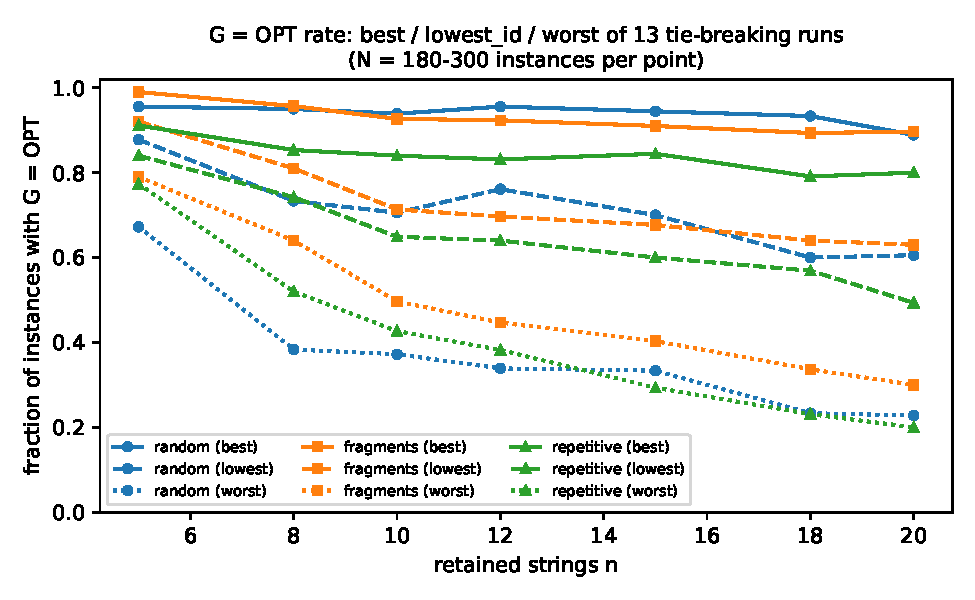
\includegraphics[width=0.7\textwidth]{results/deep_dive/fig_tie_best_worst.pdf}
\caption{Optimality rate of the best, the \texttt{lowest\_id} and the worst
of the 13 greedy runs per instance, by retained size $n$ (180--300
instances per point).}\label{fig:ties}
\end{figure}

\paragraph{Sequencing reads.} ERR098007 is a single-end Illumina GA\,IIx
run of 23{,}332 reads of phiX174, whose RefSeq reference NC\_001422.1 has
5{,}386\,bp. We excluded 180 reads not of length 76 and 34 containing
\str{N}, leaving 23{,}118 eligible reads, with no quality filtering or
trimming. An exact match against the circularised reference places 9{,}710
of them on the forward strand and 1{,}962 on the reverse strand; the other
11{,}446 do not occur exactly, most of them presumably because of
sequencing errors.
Local subsets draw forward-strand reads lying entirely within a random 250\,bp window
(redrawn if it holds fewer than 40 reads). Preprocessing removed 0.1\% of
unconditioned and 5.4\% of local reads, all duplicates. The median $\OPT$
was 745 for unconditioned and 210 for local subsets, and 46\% of
unconditioned subsets were tie-sensitive. The reference length is never
$\OPT$: it includes regions no sampled read covers, and reads with errors
are not substrings of it.

\paragraph{Runtime.} Median solve time over 5 random four-letter instances
with lengths 5--12 per $n$, excluding preprocessing and overlaps; each
instance was timed 5 times and contributes the median of its repeats. Greedy
is \texttt{lowest\_id}. Peak memory is in parentheses; the
pure-Python engine was capped at $n=20$.
\begin{center}\small
\begin{tabular}{rccc}
\toprule
$n$ & DP, numpy & DP, pure Python & Greedy\\
\midrule
10 & 0.81\,ms & 3.4\,ms & 23\,$\mu$s\\
15 & 9.1\,ms & 0.21\,s & 57\,$\mu$s\\
18 & 0.14\,s & 2.7\,s & 99\,$\mu$s\\
20 & 0.68\,s (162\,MB) & 11.5\,s (355\,MB) & 0.11\,ms\\
22 & 3.4\,s (0.58\,GB) & -- & 0.14\,ms\\
24 & 15.4\,s (2.4\,GB) & -- & 0.17\,ms\\
25 & refused (estimate 5.6\,GB) & -- & 0.20\,ms\\
\bottomrule
\end{tabular}
\end{center}
DP time roughly doubles or more with each added string, consistent with
$O(n^22^n)$. In the benchmark, the numpy solve at $n=20$ took 0.70\,s at
the median and at most 1.23\,s.

\paragraph{Comparison with the 2-approximation.} We implemented the
algorithm of~\cite{OAI26}, with run-time checks of the lemmas it relies on,
and ran it on all 4{,}953 instances of families (A)--(D). No check failed,
its lower bound $W$ never exceeded $\OPT$, and its output never exceeded
$2\,\OPT$. Lengths relative to $\OPT$ (mean / max, or mean only), where
``worst run'' is the longest of the 13 greedy runs of an instance:
\begin{center}\small
\begin{tabular}{lrcccc}
\toprule
Family & Inst. & 2-approx. & $W/\OPT$ & \texttt{lowest\_id} & Worst run\\
\midrule
Random & 1{,}260 & 1.281 / 1.897 & 0.991 & 1.009 & 1.022 / 1.222\\
Fragments & 2{,}100 & 1.259 / 1.800 & 0.983 & 1.010 & 1.022 / 1.583\\
Repetitive & 1{,}575 & 1.270 / 1.824 & 0.981 & 1.017 & 1.031 / 1.435\\
\bottomrule
\end{tabular}
\end{center}
It was longer than every greedy run on 4{,}868 instances and shorter than
the best greedy run only on four instances of $S_k$, where it stays at
$\OPT+2$ while greedy approaches $2\,\OPT$. On $S_{10,9}$ it outputs 387
($1.870\,\OPT$) against 415 for Shibata's prescribed execution. $W$ equalled
$\OPT$ on 62\% of the instances, so a greedy run of length $W$ is certified
optimal without the DP.

\paragraph{Worst-case search.} A random search over 300{,}000 binary
instances with 3--6 strings of length 2--6 found at worst the ratio
$11/7\approx1.571$ for each deterministic rule. The search is not
exhaustive: $S_5$ with $\str{c}=\str{a}$, that is \str{ABBBBB},
\str{BBBBBB}, \str{BBBBBA}, lies in the same space and has ratio $13/8$
under \texttt{lowest\_id}, but was not sampled. The seven instances kept
form the discovered part of family~(D). Four of them are exactly $S_3$ or
$S_4$ of Section~\ref{sec:compression} with $\str{c}=\str{a}$, up to
swapping \str{A} and \str{B}; the other three are small variations with a
longer end block or an extra string.

\subsection{Reproducibility}\label{app:repro}
All experiments ran on Windows~11 with an AMD Ryzen~9 9950X3D (16 cores,
32 threads) and 31\,GB of RAM, under CPython~3.14.7 with numpy~2.5.4 and
matplotlib~3.11.2, single-process on an otherwise idle machine. All
generators derive per-instance seeds from the master seed 20261105, and
tie-breaking seeds are kept separate from instance seeds. Each result
directory stores the generated instances, raw results in JSONL, a manifest
with the configuration hash, seeds and package versions, and selected merge
traces. From the repository root:
\begin{itemize}
\item \texttt{python -m pytest -q}: the correctness gate (139 tests);
\item \texttt{bash scripts/reproduce.sh}: tests, worst-case search,
  benchmark, DP scaling, analysis, the Shibata reproduction and the
  2-approximation comparison (about 15--20 minutes on one core);
\item \texttt{bash scripts/reproduce\_bio.sh}: bounded download (5\,MB cap)
  and checksummed extraction of the phiX174 data, the read experiment and
  the combined analysis.
\end{itemize}
Outputs are written to \texttt{results/standard}, \texttt{results/bio},
\texttt{results/scaling}, \texttt{results/shibata},
\texttt{results/two\_approx} and \texttt{results/deep\_dive}.

\end{document}



